\documentclass[10pt,letterpaper]{article}
\usepackage[spanish,es-tabla,es-nodecimaldot]{babel}
\usepackage[utf8]{inputenc}
\usepackage[T1]{fontenc}
\usepackage{lmodern}
\usepackage{amsmath,amssymb,amsfonts}
\usepackage{graphicx}
\usepackage{textcomp}
\usepackage{xcolor}
\usepackage{booktabs}
\usepackage{float}
\usepackage{placeins}
\usepackage{array}
\usepackage{siunitx}
\sisetup{output-decimal-marker={.},group-separator={\,},group-minimum-digits=4,detect-all}
\usepackage{url}
\usepackage{xurl}
\usepackage{etoolbox}
\usepackage{caption}
\captionsetup{font=small,labelfont=bf}
\AtBeginEnvironment{thebibliography}{\raggedright}
\usepackage{geometry}
\geometry{letterpaper,left=25mm,right=25mm,top=30mm,bottom=25mm}
\usepackage{fancyhdr}
\pagestyle{fancy}
\fancyhf{}
\rhead{EL-5854 Sistemas Fotovoltaicos}
\lhead{ITCR $\vert$ Escuela de Ingeniería Electrónica}
\rfoot{Pág.\ \thepage}
\lfoot{II Semestre 2026}
\setlength{\headheight}{14pt}
\graphicspath{{figuras/}}
\newlength{\anchofig}\setlength{\anchofig}{0.72\textwidth}
\newcommand{\kwhmd}{kWh/(m\textsuperscript{2}$\cdot$día)}
\newenvironment{IEEEkeywords}{\par\smallskip\noindent\textbf{Palabras clave:} }{\par}
\renewcommand{\thetable}{\arabic{table}}

\renewcommand{\topfraction}{0.9}
\renewcommand{\bottomfraction}{0.8}
\renewcommand{\textfraction}{0.07}
\renewcommand{\floatpagefraction}{0.75}
\setcounter{topnumber}{3}
\setcounter{bottomnumber}{2}
\setcounter{totalnumber}{4}
\let\figorig\figure \let\endfigorig\endfigure
\renewenvironment{figure}[1][]{\figorig[!htbp]}{\endfigorig}
\let\taborig\table \let\endtaborig\endtable
\renewenvironment{table}[1][]{\taborig[!htbp]}{\endtaborig}
\renewenvironment{figure*}[1][]{\begin{figure}}{\end{figure}}
\renewenvironment{table*}[1][]{\begin{table}}{\end{table}}

\begin{document}

\title{Diseño de un sistema fotovoltaico conectado a red para un establecimiento de CoopeAgri R.L. en Pérez Zeledón}
\author{A. López, S. Rojas, J. Segura\\[2pt]
\small Escuela de Ingeniería Electrónica, Instituto Tecnológico de Costa Rica}
\date{II Semestre 2026}
\thispagestyle{fancy}
\maketitle
\thispagestyle{fancy}

\begin{abstract}
En este proyecto se diseñó un sistema fotovoltaico conectado a la red para reducir la factura eléctrica del edificio de Servicios Complementarios de CoopeAgri R.L., en Pérez Zeledón, que consume \SI{223}{MWh} al año con la tarifa T-CO. A partir de las facturas, los datos solares de \textit{NASA POWER} y \textit{PVGIS} y las fichas técnicas de los equipos, la potencia se dimensionó para cubrir el consumo anual con medición neta sencilla. El sistema propuesto tiene \SI{168.3}{kWp}, con 374 módulos inclinados \SI{10}{\degree} hacia el sur y cinco inversores trifásicos de \SI{25}{kW}. El diseño incluye además la estructura de montaje, el cableado, las protecciones y el diagrama unifilar. Se estima que generaría \SI{219.5}{MWh} al año, el 98.4\,\% del consumo, y que reduciría la factura en ¢14.53 millones anuales (66.4\,\%). Con un precio estimado de ¢119.0 millones, pagando de contado y sin aumento de tarifas, la inversión se recuperaría en 9.2 años, con una TIR de 9.7\,\%.
\end{abstract}

\begin{IEEEkeywords}
sistema fotovoltaico, conexión a red, dimensionamiento, inversor, evaluación económica
\end{IEEEkeywords}

\section{Introducción}

El objetivo de este proyecto es diseñar un sistema fotovoltaico conectado a la red que reduzca la compra de energía eléctrica del edificio de Servicios Complementarios de CoopeAgri R.L., en Pérez Zeledón. La potencia del sistema se dimensionó para que la generación anual cubra el consumo del establecimiento sin superarlo, aprovechando la medición neta sencilla para recuperar en otros momentos la energía que no se consume cuando se produce. También se evaluaron cuatro potencias menores para comparar sus costos y resultados con los del sistema elegido.

El diseño parte del consumo registrado en las facturas del último año, de los datos de radiación y temperatura del sitio y de las fichas técnicas de los equipos seleccionados.


\section{Descripción del lugar de estudio}\label{sec:lugar}

El establecimiento es el edificio de Servicios Complementarios de la Cooperativa Agrícola Industrial y de Servicios Múltiples El General (CoopeAgri R.L.), en San Isidro de El General, Pérez Zeledón. Su servicio eléctrico corresponde al NISE 2471778 del Instituto Costarricense de Electricidad (ICE) \cite{ice_facturas}. La Tabla~\ref{tab:sitio} resume la información general del sitio.

\begin{table}[!htb]
\caption{Información general del sitio}
\label{tab:sitio}
\centering
\footnotesize
\setlength{\tabcolsep}{3pt}
\begin{tabular}{l l}
\toprule
Parámetro & Valor \\
\midrule
Servicio & CoopeAgri R.L., Servicios Complementarios \\
NISE / medidor & 2471778 / 2092972 \\
Ubicación & San Isidro de El General, Pérez Zeledón \\
Coordenadas & \ang{9;22;37.0}\,N, \ang{83;42;6.8}\,O \\
Elevación & \SI{704}{m} s.\,n.\,m. \\
Tarifa & T-CO (comercio y servicios), no horaria \\
Acometida & Trifásica, 120/\SI{208}{V} \\
Techo disponible & \SI{1990}{m^2}, lámina metálica, $\approx\SI{0}{\degree}$ \\
Orientación del techo & Eje largo a $\approx\SI{7}{\degree}$ del norte--sur \\
Horario de atención & Lunes a sábado, 6:00 a 21:00 \\
\bottomrule
\end{tabular}
\end{table}

\subsection{Características de la zona}

San Isidro de El General está en el valle de El General, en la vertiente del Pacífico sur. La temperatura media mensual se mantiene entre \SI{21}{\celsius} y \SI{23}{\celsius}, y los extremos horarios entre 2005 y 2025 van de \SI{14.1}{\celsius} a \SI{30.5}{\celsius} \cite{nasa_power, nasa_power_horario}; estos valores se usan en la Sección~\ref{sec:modulo} para calcular las tensiones extremas de las cadenas. Hay una época seca de diciembre a abril y una lluviosa, con más nubosidad, de mayo a noviembre.

\subsection{Ubicación (vista satelital)}

La Fig.~\ref{fig:ubicacion} muestra la ubicación del edificio, en el sector norte del centro de San Isidro.

\begin{figure}[!htb]
\centering
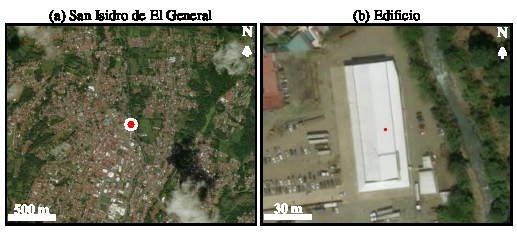
\includegraphics[width=\anchofig]{ubicacion_satelital.pdf}
\caption{Vista satelital del sitio de estudio ($9.37695^\circ$~N, $83.70189^\circ$~O): (a) ubicación en San Isidro de El General; (b) edificio de Servicios Complementarios (punto rojo).}
\label{fig:ubicacion}
\end{figure}

\subsection{Techo disponible}

Para el diseño se considera la parte central y más alta de la cubierta, de lámina metálica, con un área de \SI{1990}{m^2} y una inclinación cercana a \SI{0}{\degree}. A partir de la imagen satelital, esta superficie mide aproximadamente \SI{21.5}{m} de este a oeste y \SI{92.5}{m} de norte a sur. El eje largo del techo no está exactamente en la dirección norte--sur: en la imagen está girado unos \SI{7}{\degree}, con su extremo sur desplazado hacia el este. Por ser la parte más alta del edificio, no recibe sombra de los niveles más bajos de la cubierta.

\subsection{Caracterización del consumo eléctrico}

El servicio está en la tarifa T-CO, que cobra por separado la energía consumida y la demanda máxima del mes. La Tabla~\ref{tab:consumo} y la Fig.~\ref{fig:consumo} presentan los doce meses de setiembre de 2025 a agosto de 2026 \cite{ice_facturas}.

\begin{table}[!htb]
\caption{Consumo, demanda, factor de potencia y monto facturado (set.\ 2025 -- ago.\ 2026)}
\label{tab:consumo}
\centering
\footnotesize
\setlength{\tabcolsep}{3.5pt}
\begin{tabular}{l S[table-format=6.0] S[table-format=2.2] S[table-format=1.2] S[table-format=8.0]}
\toprule
{Mes} & {Energía [kWh]} & {Demanda [kW]} & {F.P.} & {Monto [¢]} \\
\midrule
Set. 2025 & 18238 & 53.00 & 0.95 & 2197090 \\
Oct. 2025 & 18727 & 47.12 & 0.98 & 2160335 \\
Nov. 2025 & 17993 & 44.92 & 0.98 & 2071120 \\
Dic. 2025 & 18972 & 44.31 & 0.98 & 2143700 \\
Ene. 2026 & 18482 & 43.70 & 0.96 & 1784895 \\
Feb. 2026 & 17626 & 49.33 & 0.98 & 1787605 \\
Mar. 2026 & 18238 & 45.78 & 0.98 & 1790965 \\
Abr. 2026 & 18850 & 46.14 & 0.98 & 1837895 \\
May. 2026 & 19339 & 46.88 & 0.98 & 1880430 \\
Jun. 2026 & 18482 & 45.78 & 0.98 & 1808075 \\
Jul. 2026 & 18972 & 44.19 & 0.98 & 1824720 \\
Ago. 2026 & 19094 & 47.25 & 0.98 & 1867375 \\
\midrule
Total     & 223013 & {--} & {--} & 23154205 \\
Promedio  & 18584  & 46.53 & {--} & 1929517 \\
\bottomrule
\end{tabular}
\end{table}

\begin{figure}[!htb]
\centering
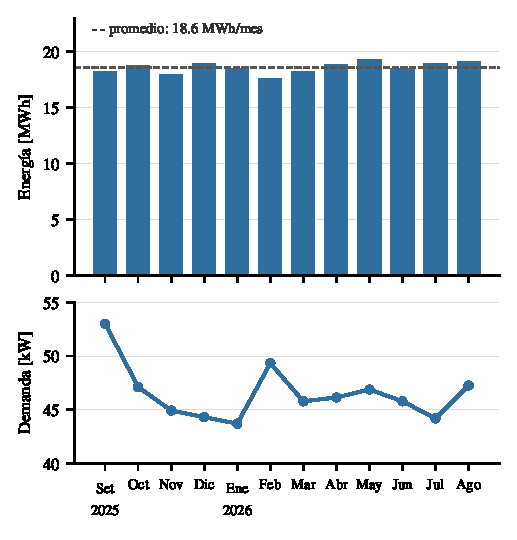
\includegraphics[width=\anchofig]{consumo_mensual.pdf}
\caption{Energía consumida (arriba) y demanda máxima (abajo) por mes de facturación.}
\label{fig:consumo}
\end{figure}

El consumo anual fue de \SI{223013}{kWh}, con un promedio de \SI{18584}{kWh} por mes. La variación entre meses es pequeña (desviación estándar del 2.7\,\%), así que las diferencias entre la generación y el consumo de cada mes dependerán casi solo de la radiación solar. Algunos valores de la Tabla~\ref{tab:consumo} se repiten porque todos los registros son múltiplos de la constante del medidor (\SI{122.4}{kWh}). La demanda máxima estuvo entre \SI{43.7}{kW} y \SI{53.0}{kW}.

En agosto de 2026 la energía representó el 61\,\% del monto facturado, la demanda el 25\,\%, el impuesto de valor agregado el 11\,\%, y el alumbrado público y el tributo de bomberos el 3\,\% restante \cite{ice_facturas}. Como el cargo por demanda depende de la demanda máxima del mes, el sistema no necesariamente lo reduce aunque disminuya la energía comprada; por eso, en el caso base de la evaluación económica se supone que no cambia.

\section{Recurso solar}\label{sec:recurso}

\subsection{Diagramas cilíndricos del sitio}

La posición del Sol se describe con dos ángulos: la altura solar $h$, medida desde el plano horizontal, y el acimut $\alpha$, medido sobre el horizonte. En este trabajo el acimut se mide desde el norte y en sentido horario (\SI{90}{\degree} al este, \SI{180}{\degree} al sur).

Para calcular estos ángulos se trabajó con el tiempo solar $t_s$, que se obtiene a partir de la hora local $t_u$ con
\begin{equation}
t_s = t_u + \frac{L - L_R}{15} + \Delta_{\mathrm{eot}},
\label{eq:ts}
\end{equation}
donde $L=\SI{-83.70}{\degree}$ es la longitud del sitio, $L_R=\SI{-90}{\degree}$ es la longitud de referencia de Costa Rica y $\Delta_{\mathrm{eot}}$ es la ecuación del tiempo, en horas. Con este resultado el mediodía solar ocurre entre las 11:18 y las 11:49, hora local, según la época del año.

El ángulo horario $\omega$, la declinación $\delta$, la altura solar $h$ y el acimut $\alpha_S$ se calcularon con
\begin{align}
\omega &= 15\,(t_s - 12), \label{eq:omega}\\
\delta &= \sin^{-1}\!\big[0.3978\sin\!\big(\bar d - 1.400 \nonumber\\ &\qquad + 0.0355\sin(\bar d - 0.0489)\big)\big], \label{eq:decl}\\
\sin h &= \sin\varphi\,\sin\delta + \cos\varphi\,\cos\delta\,\cos\omega, \label{eq:altura}\\
\sin \alpha_S &= \frac{\cos\delta\,\sin\omega}{\cos h}, \label{eq:acimut}
\end{align}
donde $\varphi=\SI{9.377}{\degree}$ es la latitud y $\bar d = 2\pi d/365.25$ el ángulo diario, en radianes, con $d$ el día del año ($d=1$ el 1 de enero). El acimut de \eqref{eq:acimut} se mide desde el sur; cuando el Sol pasa al norte del cenit se corrigió el cuadrante y el resultado se refirió al norte.

La Fig.~\ref{fig:cilindrico} presenta el diagrama cilíndrico del sitio para el día 21 de cada mes, calculado con estas ecuaciones. La Fig.~\ref{fig:cilindrico_uo} muestra el diagrama obtenido con la herramienta de la Universidad de Oregon para las mismas coordenadas \cite{uoregon}. Las trayectorias y las alturas máximas coinciden con las calculadas; las líneas de hora aparecen desplazadas porque esa herramienta usa la hora estándar local y no la hora solar.

\begin{figure*}[!t]
\centering
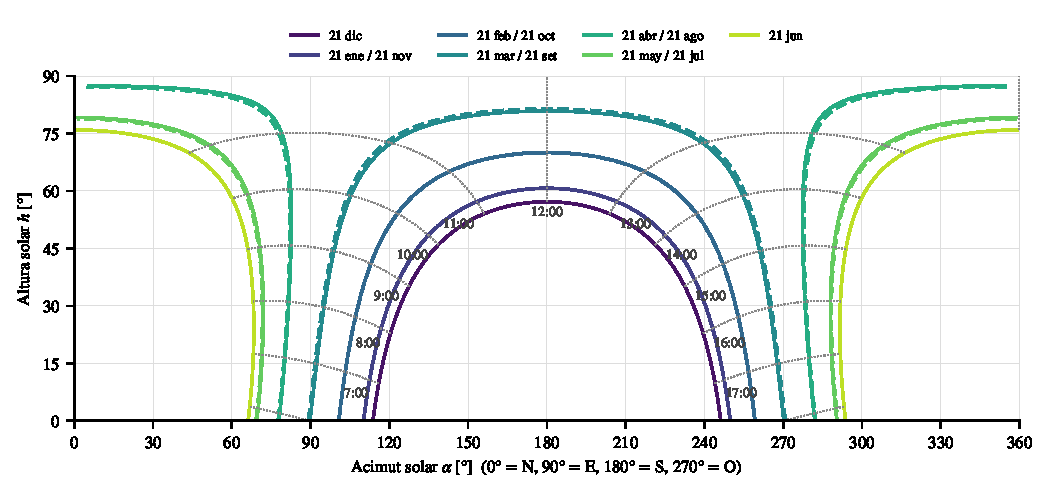
\includegraphics[width=0.85\textwidth]{diagrama_cilindrico.pdf}
\caption{Diagrama cilíndrico del recorrido solar en San Isidro de El General (\SI{9.377}{\degree}\,N), día 21 de cada mes, en tiempo solar. Las líneas punteadas unen puntos de la misma hora.}
\label{fig:cilindrico}
\end{figure*}

\begin{figure*}[!t]
\centering
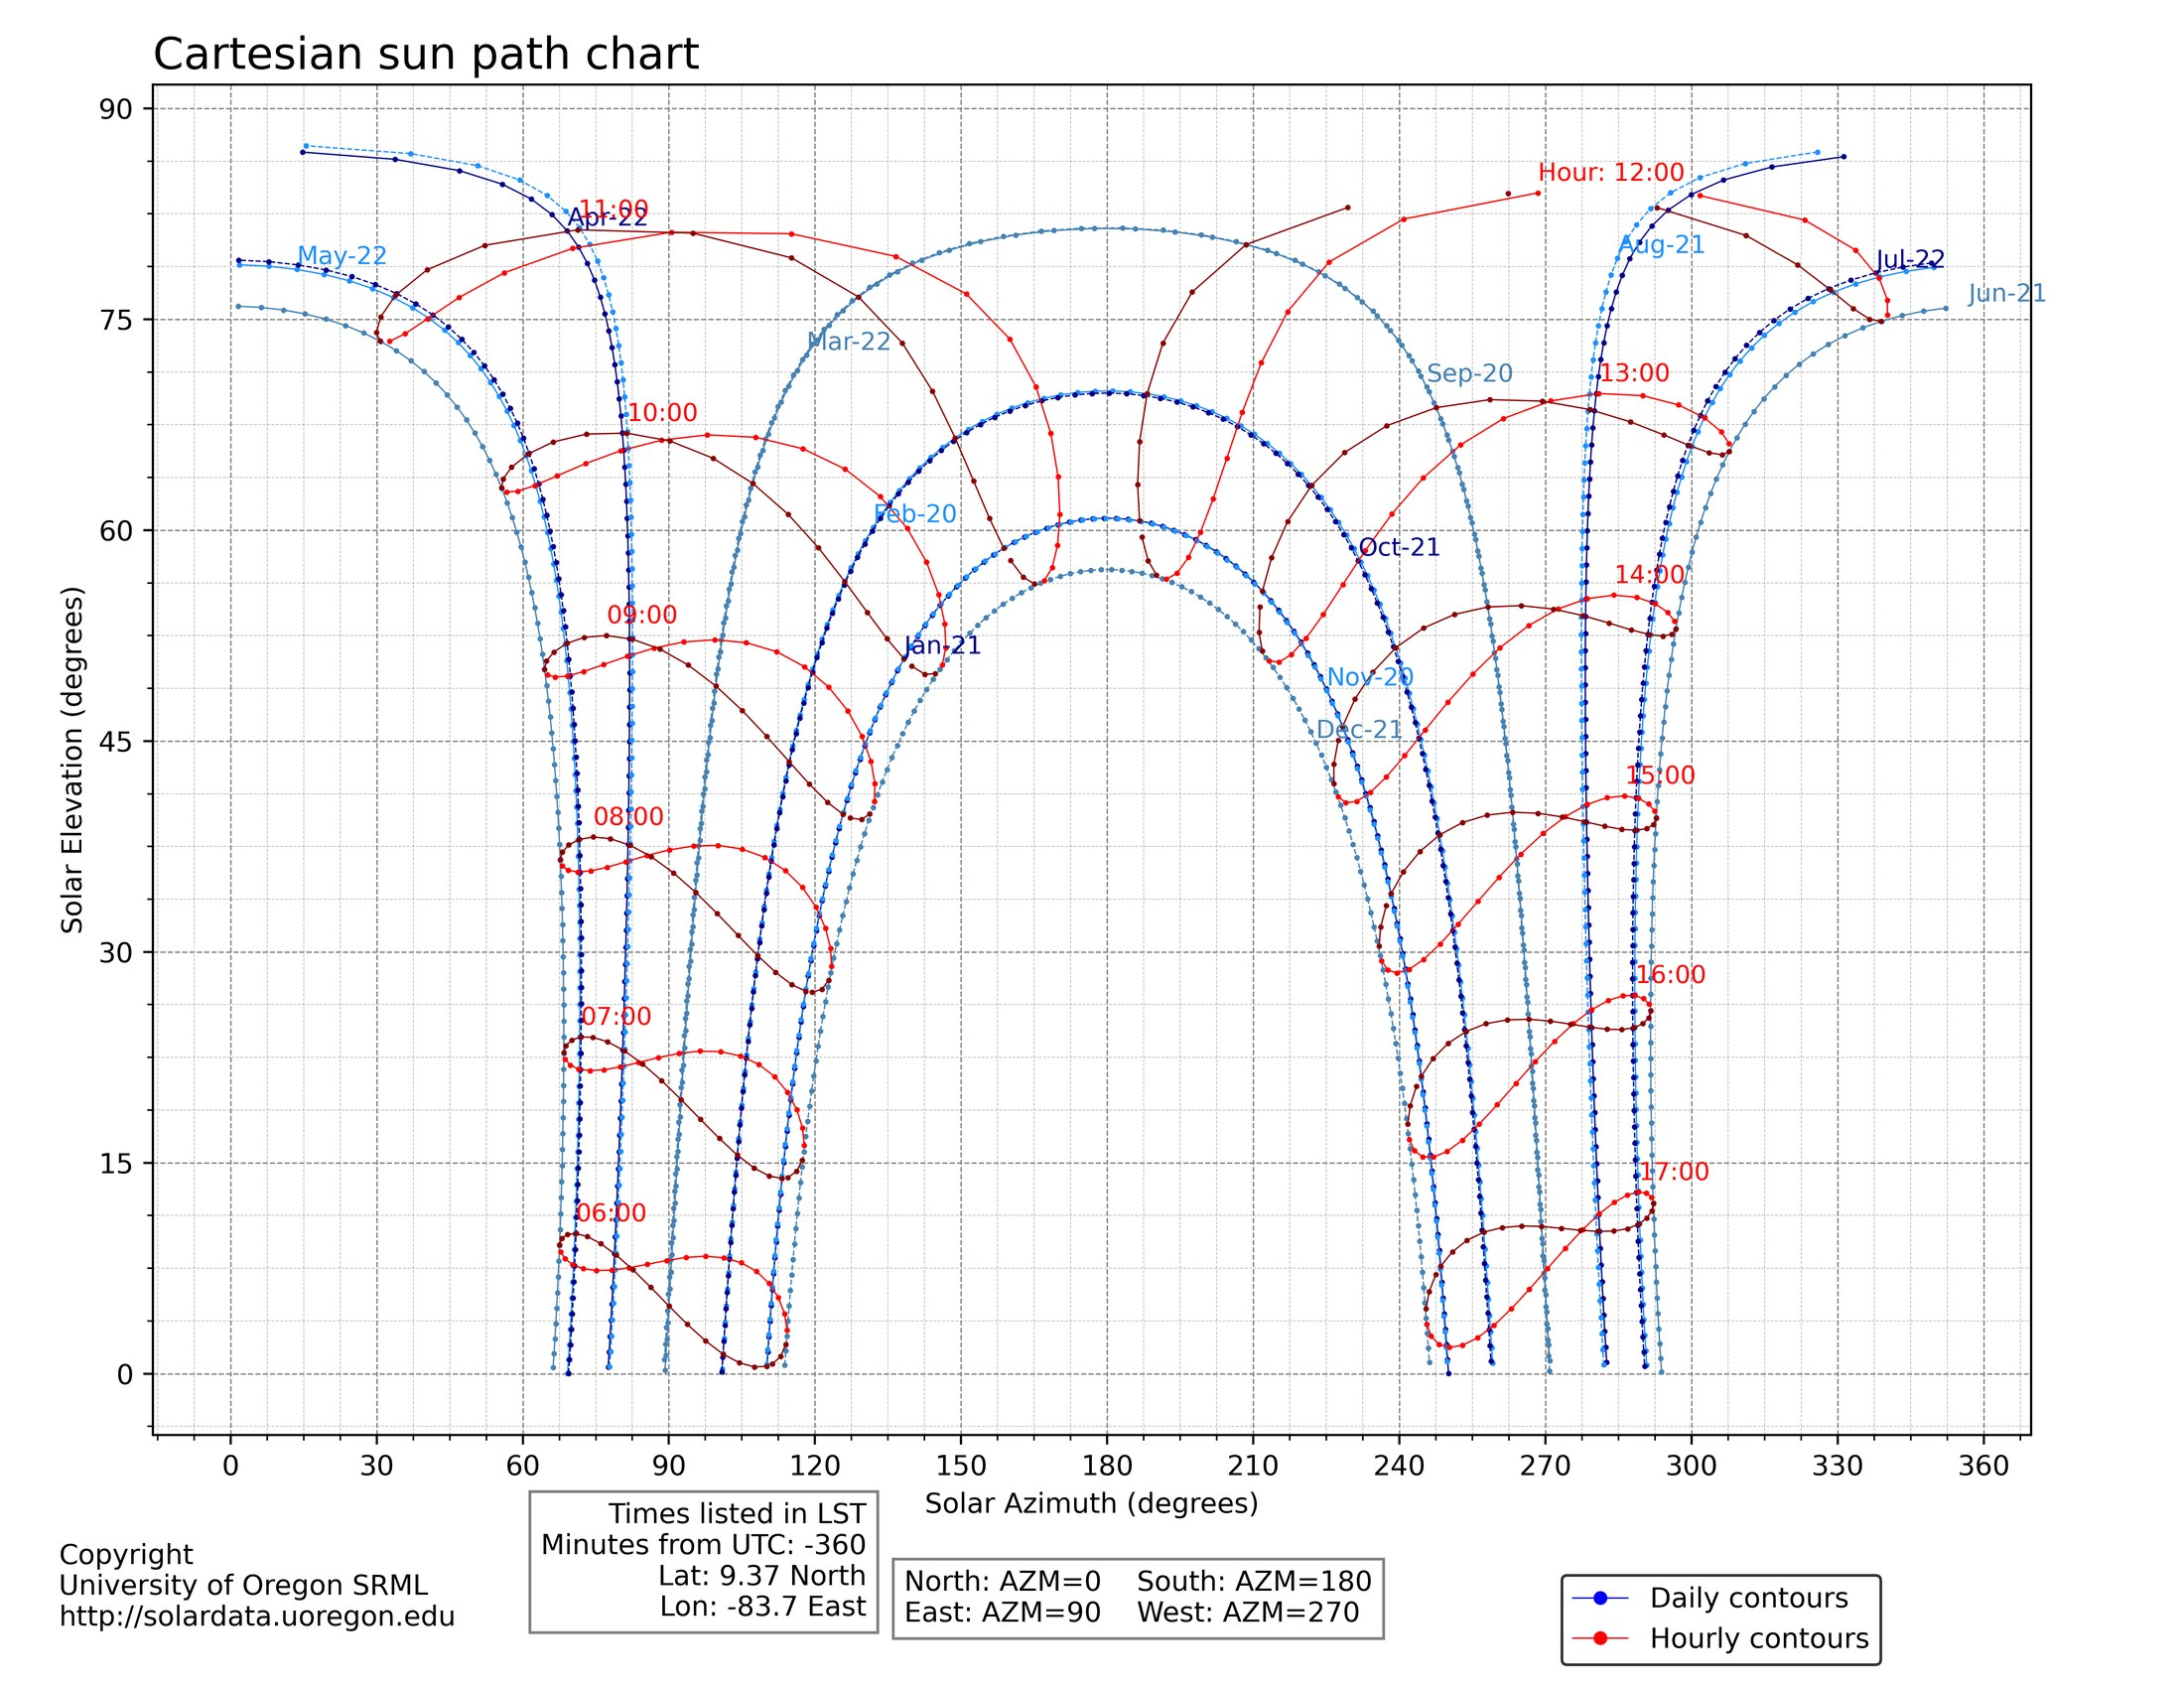
\includegraphics[width=0.72\textwidth]{cilindrico_uoregon.jpg}
\caption{Diagrama cilíndrico del sitio generado con la herramienta de la Universidad de Oregon, en hora estándar local (UTC$-6$) \cite{uoregon}.}
\label{fig:cilindrico_uo}
\end{figure*}

Por la cercanía al ecuador, el Sol pasa muy alto todo el año: al mediodía solar la altura no baja de \SI{57.2}{\degree} (21 de diciembre), y entre mediados de abril y finales de agosto el Sol pasa al norte del cenit. La duración del día también cambia poco, entre \SI{11.45}{h} y \SI{12.55}{h}. Diciembre presenta las menores alturas: a las 10:00 y a las 14:00 (hora solar) del 21 de diciembre la altura es de \SI{46.0}{\degree}, valor que se usa para calcular la separación entre filas de módulos.

\subsection{Componentes de radiación y bases de datos meteorológicas usadas}

La radiación global horizontal (GHI) es la suma de la componente difusa horizontal (DHI) y de la directa proyectada sobre el plano horizontal. Las bases de datos reportan la directa sobre un plano perpendicular a los rayos (DNI), por lo que la GHI no es igual a la suma de la DNI y la DHI, sino que
\begin{equation}
\mathrm{GHI} = \mathrm{DHI} + \mathrm{DNI}\cos\theta_z, \label{eq:ghi}
\end{equation}
donde $\theta_z = \SI{90}{\degree}-h$ es el ángulo cenital. Sobre un plano inclinado se suma una tercera componente, la reflejada por el suelo, que depende del albedo. Con \SI{10}{\degree} de inclinación el módulo casi no ve el suelo: el factor $(1-\cos\beta)/2$ vale 0.008, de modo que con un albedo típico de 0.2 esta componente aporta menos del 0.2\,\% de la GHI.

Se utilizaron dos bases de datos satelitales y, como comprobación, mediciones históricas del Instituto Meteorológico Nacional (IMN):
\begin{itemize}
\item \textbf{\textit{NASA POWER}} \cite{nasa_power}: promedios mensuales de 2001 a 2025 de radiación (estimada desde satélite) y de temperatura. Es la base usada en el diseño.
\item \textbf{\textit{PVGIS} 5.3} \cite{pvgis}: base \textit{PVGIS}-ERA5, promedios de 2005 a 2023 obtenidos de un reanálisis meteorológico. Se usa como comparación.
\item \textbf{IMN} \cite{imn_castro}: radiación global media de la estación Repunta, en Pérez Zeledón (\ang{9;18;}\,N, \ang{83;39;}\,O, \SI{580}{m}), estimada con el brillo solar de 1962 a 1980. Se usa como comprobación.
\end{itemize}
La Tabla~\ref{tab:radiacion} presenta la irradiación diaria promedio de cada mes en \kwhmd; en esta unidad la GHI coincide con las horas solares pico (HSP) sobre el plano horizontal.

\begin{table}[!htb]
\caption{Irradiación diaria promedio mensual [\kwhmd]}
\label{tab:radiacion}
\centering
\small
\setlength{\tabcolsep}{4pt}
\begin{tabular}{l S[table-format=1.2] S[table-format=1.2] S[table-format=1.2] S[table-format=1.2] S[table-format=-2.1]}
\toprule
 & \multicolumn{3}{c}{\textit{NASA POWER}} & {\textit{PVGIS}} & {Dif.} \\
\cmidrule(lr){2-4}
{Mes} & {GHI} & {DNI} & {DHI} & {GHI} & {[\%]} \\
\midrule
Ene & 4.56 & 4.40 & 1.67 & 5.22 & 14.6 \\
Feb & 5.10 & 4.63 & 1.83 & 5.85 & 14.9 \\
Mar & 5.30 & 4.19 & 2.04 & 5.99 & 13.1 \\
Abr & 4.82 & 2.79 & 2.29 & 5.36 & 11.2 \\
May & 4.35 & 2.00 & 2.32 & 4.31 & -0.9 \\
Jun & 4.30 & 1.74 & 2.44 & 4.09 & -5.0 \\
Jul & 4.17 & 1.67 & 2.38 & 4.15 & -0.5 \\
Ago & 4.30 & 1.79 & 2.39 & 4.18 & -2.8 \\
Set & 4.47 & 2.16 & 2.35 & 4.14 & -7.4 \\
Oct & 4.03 & 1.95 & 2.18 & 3.69 & -8.3 \\
Nov & 3.68 & 2.30 & 1.87 & 3.70 & 0.7 \\
Dic & 4.07 & 3.66 & 1.67 & 4.57 & 12.1 \\
\midrule
Prom. & 4.42 & 2.76 & 2.12 & 4.60 & 3.9 \\
\bottomrule
\end{tabular}
\\[2pt]
{\footnotesize Dif.: diferencia de la GHI de \textit{PVGIS} respecto a \textit{NASA POWER}.}
\end{table}

Según \textit{NASA POWER}, la DNI es mayor de diciembre a marzo y la GHI de enero a abril, mientras que de mayo a noviembre la componente difusa supera el 50\,\% de la global (Fig.~\ref{fig:radiacion}). Los valores anuales son de \SI{1615}{kWh/m^2} con \textit{NASA POWER} y \SI{1678}{kWh/m^2} con \textit{PVGIS}, una diferencia de 3.9\,\%. La diferencia se concentra en la época seca, cuando \textit{PVGIS} da entre 11 y 15\,\% más, posiblemente porque ambas bases estiman la nubosidad de forma distinta. La estación Repunta del IMN tiene un promedio de \SI{16}{MJ/m^2} por día, es decir, 4.4~\kwhmd \cite{imn_castro}, prácticamente igual al de \textit{NASA POWER} (4.42). Por eso el diseño se basa en \textit{NASA POWER}: coincide con la estación del IMN, cubre un período más largo y, al dar el valor más bajo, evita sobrestimar la generación.

\begin{figure}[!htb]
\centering
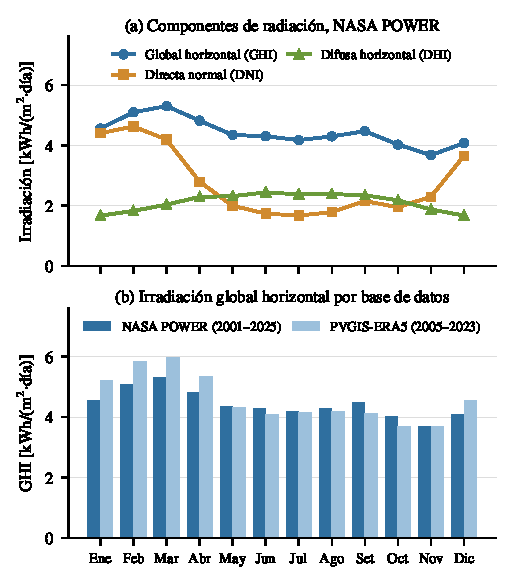
\includegraphics[width=\anchofig]{radiacion_componentes.pdf}
\caption{(a) Componentes de radiación mensuales según \textit{NASA POWER}. (b) Comparación de la irradiación global horizontal entre \textit{NASA POWER} y \textit{PVGIS}.}
\label{fig:radiacion}
\end{figure}

Los promedios mensuales ocultan la variación que existe de un día a otro. Para observarla se consultaron en \textit{NASA POWER} las series diarias de 2025 de las tres componentes en cielo real, es decir, incluyendo el efecto de las nubes \cite{nasa_power_diario}. En la Fig.~\ref{fig:diaria} se observa que un día cualquiera puede alejarse bastante del promedio del mes. La directa normal es la más sensible a las nubes: es alta de diciembre a marzo y cae de forma marcada de mayo a noviembre, mientras que la difusa es más estable y gana peso en la época lluviosa, cuando sostiene la producción en días nublados. El promedio de 2025 fue de 4.31~\kwhmd, un 2.5\,\% menor que el promedio de largo plazo usado para el diseño, lo que muestra que la producción de un año particular puede variar algunos puntos respecto a la estimación.

\begin{figure}[!htb]
\centering
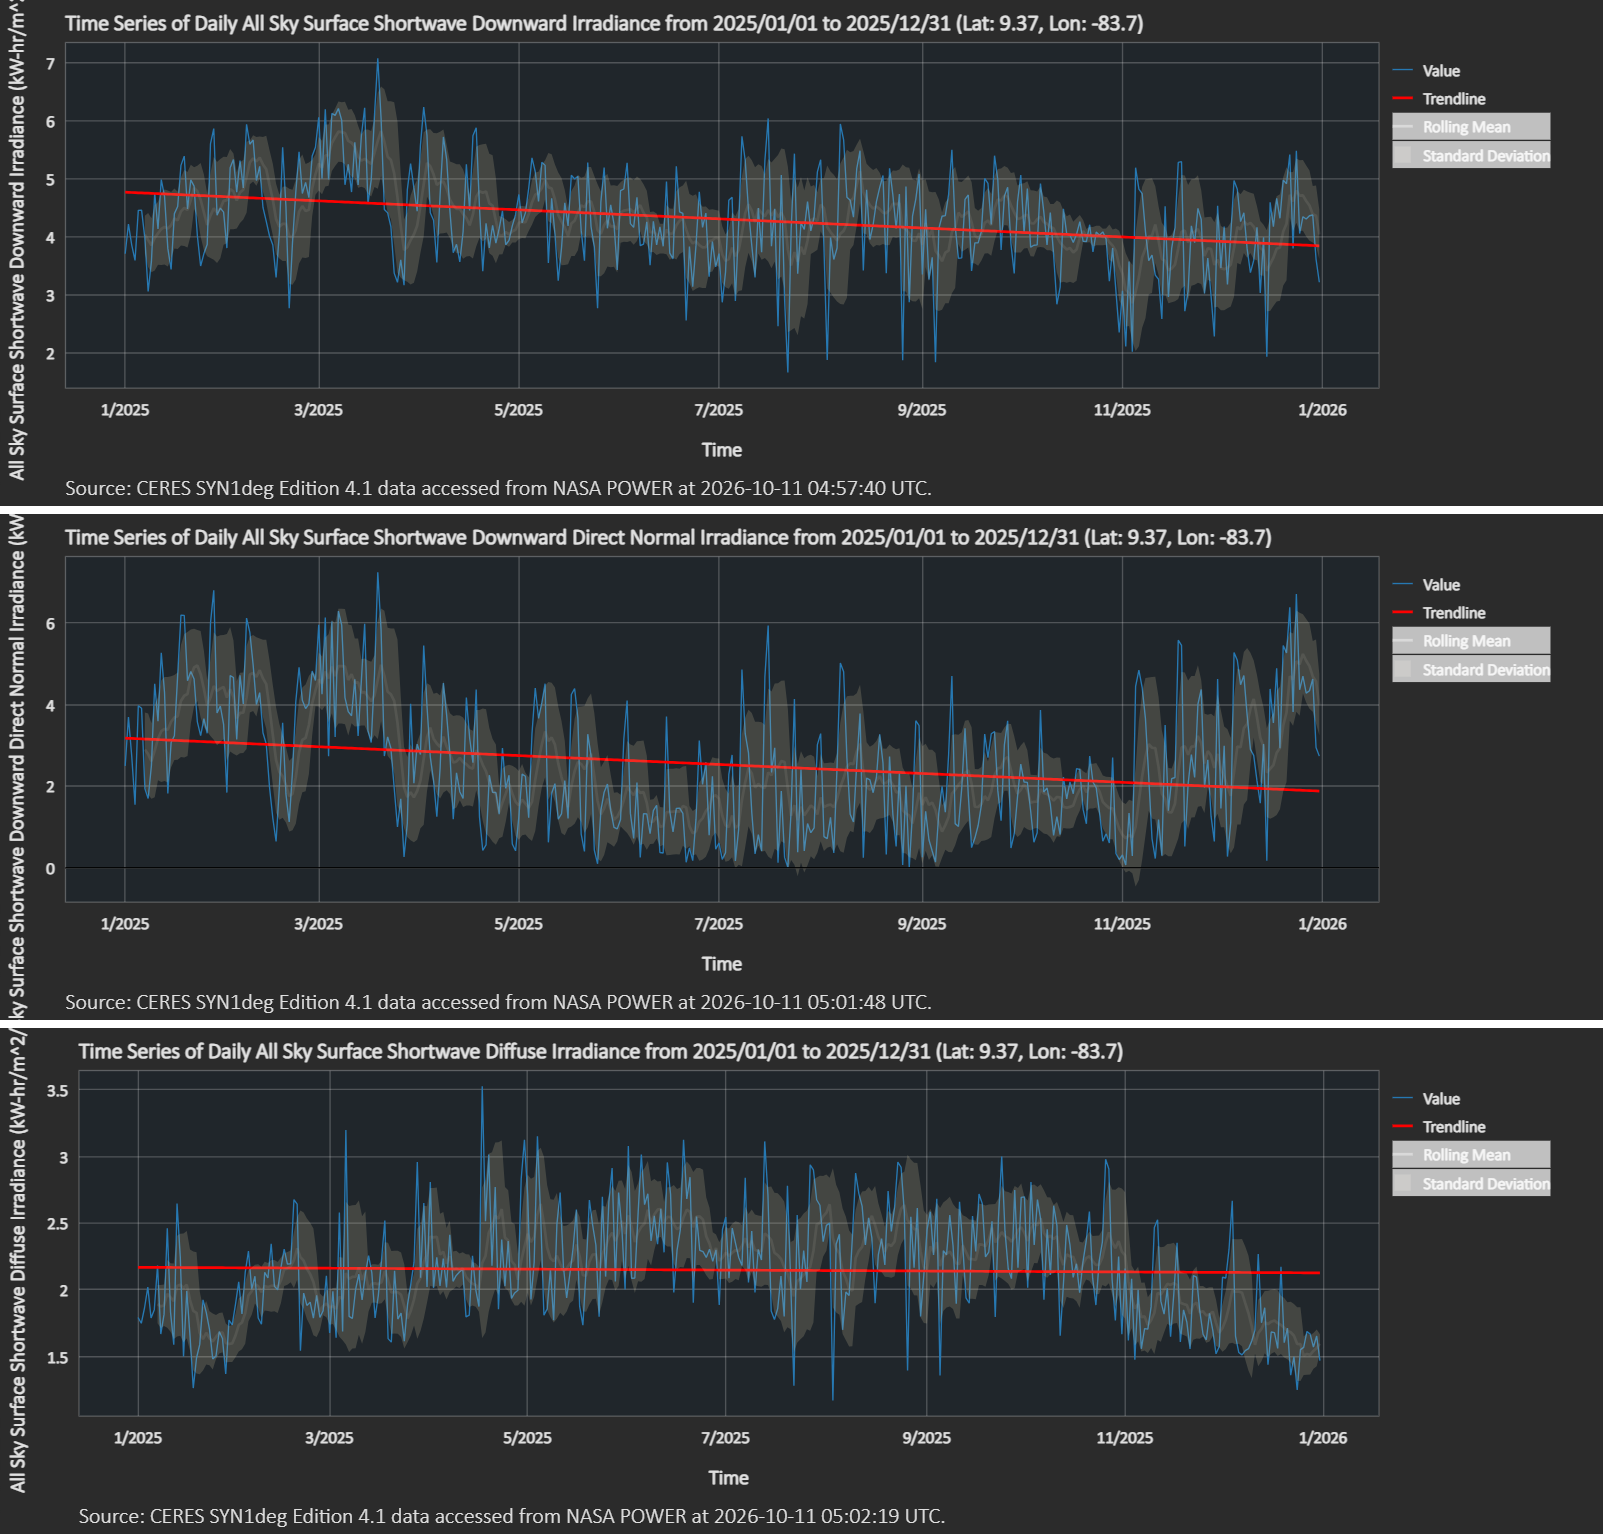
\includegraphics[width=\anchofig,height=0.4\textheight,keepaspectratio]{irradiacion_diaria_2025.png}
\caption{Irradiación diaria en 2025 según \textit{NASA POWER}: (a) global horizontal, (b) directa normal y (c) difusa horizontal, en kWh/(m\textsuperscript{2}$\cdot$día). La línea roja es la tendencia lineal de cada serie \cite{nasa_power_diario}.}
\label{fig:diaria}
\end{figure}

\subsection{Cálculo del ángulo óptimo y comparación con el ángulo disponible}

La radiación sobre un plano inclinado se estimó con los factores de corrección $K$ para una latitud de \SI{10}{\degree}, la más cercana a la del sitio \cite{factores_k}:
\begin{equation}
H_{\beta} = K_{\beta}\,H_{h},
\label{eq:k}
\end{equation}
donde $H_h$ es la irradiación global horizontal y $K_\beta$ el factor para una inclinación $\beta$ hacia el sur. La Tabla~\ref{tab:inclinacion} y la Fig.~\ref{fig:inclinacion} presentan la irradiación anual para las inclinaciones evaluadas.

\begin{table}[!htb]
\caption{Irradiación anual sobre el plano inclinado (orientación sur)}
\label{tab:inclinacion}
\centering
\small
\begin{tabular}{S[table-format=2.0] S[table-format=4.0] S[table-format=-2.1] S[table-format=4.0]}
\toprule
{$\beta$ [°]} & {NASA [kWh/m\textsuperscript{2}]} & {Var. [\%]} & {\textit{PVGIS} [kWh/m\textsuperscript{2}]} \\
\midrule
0  & 1615 & 0.0  & 1678 \\
5  & 1628 & 0.8  & 1692 \\
10 & 1625 & 0.6  & 1691 \\
15 & 1616 & 0.0  & 1682 \\
20 & 1594 & -1.3 & 1661 \\
25 & 1562 & -3.3 & 1629 \\
30 & 1523 & -5.7 & 1589 \\
\bottomrule
\end{tabular}
\\[2pt]
{\footnotesize Var.: variación respecto al plano horizontal con datos de \textit{NASA POWER}.}
\end{table}

\begin{figure}[!htb]
\centering
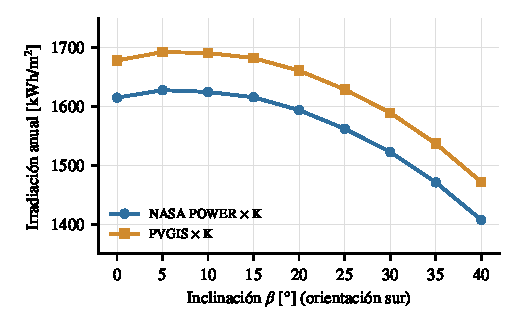
\includegraphics[width=\anchofig]{inclinacion_anual.pdf}
\caption{Irradiación anual en función de la inclinación, con los factores $K$ aplicados a cada base de datos.}
\label{fig:inclinacion}
\end{figure}

Entre los ángulos evaluados, la mayor irradiación anual se obtiene con \SI{5}{\degree}, con una ganancia de 0.8\,\% frente al plano horizontal, y con \SI{10}{\degree} es solo 0.2\,\% menor. Inclinar los módulos favorece los meses de setiembre a marzo, cuando el Sol pasa por el sur, pero reduce la radiación de abril a agosto, cuando pasa por el norte. Con los datos de \textit{PVGIS} el resultado es el mismo: el máximo también se obtiene con \SI{5}{\degree} (Tabla~\ref{tab:inclinacion}).

Como el techo es prácticamente plano, la inclinación la define la estructura. Se eligieron \SI{10}{\degree} hacia el sur en lugar del óptimo de \SI{5}{\degree}. El manual de instalación del módulo pide escoger una inclinación que evite que se acumulen agua y polvo sobre los módulos, e indica que con una inclinación suficiente la lluvia ayuda a limpiar su superficie \cite{aiko_manual}; por eso se prefirió no bajar hasta \SI{5}{\degree}. Este cambio casi no afecta la energía, porque se pierden solo \SI{3}{kWh/m^2} al año (0.2\,\%), y tampoco ocupa más techo, porque la separación adoptada entre filas, de \SI{2.5}{m}, supera la distancia mínima con cualquiera de los dos ángulos (\SI{2.03}{m} con \SI{10}{\degree} y \SI{1.90}{m} con \SI{5}{\degree}; Sección~\ref{sec:instalacion}). Con esta inclinación la irradiación de diseño es de \SI{1625}{kWh/m^2} por año, en promedio \SI{4.45}{HSP}.

\section{Módulo fotovoltaico}\label{sec:modulo}

\subsection{Descripción del módulo y tecnología}

Se seleccionó el módulo AIKO Neostar 2S AIKO-A450-MAH54Mb, de \SI{450}{W}, por su eficiencia de 22.6\,\%, su bajo coeficiente de temperatura de potencia (\SI{-0.26}{\%/\celsius}) y su baja degradación garantizada, de 1\,\% el primer año y 0.35\,\% por año después \cite{aiko_ds}.

El módulo es de silicio monocristalino tipo n con celdas ABC (\emph{all back contact}), que tienen los dos contactos en la cara posterior; así la cara frontal no tiene rejilla metálica que haga sombra sobre la celda. El módulo está formado por 108 medias celdas, tiene vidrio templado de \SI{3.2}{mm}, marco de aluminio y tres diodos de paso \cite{aiko_ds}. El uso de medias celdas reduce la corriente en cada celda y, con ello, las pérdidas resistivas.

\subsection{Tabla resumen de características eléctricas}

La Tabla~\ref{tab:modulo} reúne los datos de la ficha técnica en condiciones estándar de prueba (STC) y NOCT. El fusible máximo en serie se usa en la Sección~\ref{sec:instalacion} para elegir los fusibles de cadena.

\begin{table}[!htb]
\caption{Características del módulo AIKO-A450-MAH54Mb \cite{aiko_ds}}
\label{tab:modulo}
\centering
\footnotesize
\setlength{\tabcolsep}{3pt}
\begin{tabular}{l c c}
\toprule
Parámetro & STC & NOCT \\
\midrule
Potencia máxima, $P_{\max}$ & \SI{450}{W} & \SI{339}{W} \\
Tensión de máx. potencia, $V_{mp}$ & \SI{33.70}{V} & \SI{31.83}{V} \\
Corriente de máx. potencia, $I_{mp}$ & \SI{13.36}{A} & \SI{10.66}{A} \\
Tensión de circuito abierto, $V_{oc}$ & \SI{40.69}{V} & \SI{38.43}{V} \\
Corriente de cortocircuito, $I_{sc}$ & \SI{14.12}{A} & \SI{11.42}{A} \\
\midrule
Eficiencia del módulo & \multicolumn{2}{c}{22.6\,\%} \\
Coef. de temperatura de $P_{\max}$ & \multicolumn{2}{c}{\SI{-0.26}{\%/\celsius}} \\
Coef. de temperatura de $V_{oc}$ & \multicolumn{2}{c}{\SI{-0.22}{\%/\celsius}} \\
Coef. de temperatura de $I_{sc}$ & \multicolumn{2}{c}{\SI[retain-explicit-plus]{+0.05}{\%/\celsius}} \\
Tensión máxima del sistema & \multicolumn{2}{c}{\SI{1500}{V} DC} \\
Fusible máximo en serie & \multicolumn{2}{c}{\SI{25}{A}} \\
Dimensiones & \multicolumn{2}{c}{\SI{1757}{} $\times$ \SI{1134}{} $\times$ \SI{30}{mm}} \\
Masa & \multicolumn{2}{c}{\SI{21.5}{kg}} \\
Cable de salida & \multicolumn{2}{c}{\SI{4}{mm^2} (12 AWG), conector MC4} \\
\bottomrule
\end{tabular}
\\[2pt]
{\footnotesize STC (\textit{Standard Test Conditions}): \SI{1000}{W/m^2}, \SI{25}{\celsius} en la celda, AM 1.5. NOCT (\textit{Nominal Operating Cell Temperature}): \SI{800}{W/m^2}, \SI{20}{\celsius} ambiente, viento de \SI{1}{m/s}. Los coeficientes de temperatura están declarados a STC.}
\end{table}

\subsection{Estimación de la variación de los parámetros eléctricos}

Los parámetros se corrigieron para la temperatura mínima de la celda, que da la mayor tensión, y para la máxima, que da la menor tensión y la menor potencia.

La temperatura de la celda se estimó con
\begin{equation}
T_{\mathrm{celda}} = T_{\mathrm{amb}} + \frac{\mathrm{NOCT}-20}{800}\,G,
\label{eq:tcelda}
\end{equation}
donde $G$ es la irradiancia en \si{W/m^2}. La ficha técnica no da la temperatura NOCT de la celda, por lo que se estimó con los valores NOCT de la Tabla~\ref{tab:modulo}. Con \SI{800}{W/m^2} y la celda a \SI{25}{\celsius}, el módulo daría \SI{360}{W} ($0.8\times\SI{450}{W}$); para que la potencia baje a los \SI{339}{W} de la ficha, según el coeficiente de potencia, la celda debe estar a \SI{47.4}{\celsius}. Con la corriente se obtiene \SI{47.0}{\celsius}. Se usó un NOCT estimado de \SI{47}{\celsius}.

La temperatura mínima de la celda se tomó igual a la mínima ambiente, \SI{14.1}{\celsius}, porque al amanecer, con muy poca irradiancia, la celda está prácticamente a la temperatura del aire. Para la máxima se usó la ambiente máxima de \SI{30.5}{\celsius} con $G=\SI{1000}{W/m^2}$, lo que según \eqref{eq:tcelda} da \SI{64.3}{\celsius}. Ambas temperaturas provienen de \textit{NASA POWER} \cite{nasa_power}.

Cada parámetro se corrigió con
\begin{equation}
X(T) = X_{\mathrm{STC}}\left[1 + \frac{\gamma_X}{100}\,(T_{\mathrm{celda}} - 25)\right],
\label{eq:correccion}
\end{equation}
donde $\gamma_X$ es el coeficiente de temperatura del parámetro en \si{\%/\celsius}. La ficha no da coeficientes para $V_{mp}$ e $I_{mp}$. Para $I_{mp}$ se usó el de $I_{sc}$, y para $V_{mp}$ se estimó $\gamma_{V_{mp}}\approx\gamma_{P}-\gamma_{I_{sc}}=\SI{-0.31}{\%/\celsius}$, de modo que el producto $V_{mp}\cdot I_{mp}$ concuerde con la potencia corregida. Este coeficiente es una aproximación y no un dato del fabricante. Los resultados se presentan en la Tabla~\ref{tab:temperatura}.

\begin{table}[!htb]
\caption{Parámetros del módulo corregidos por temperatura (\SI{1000}{W/m^2})}
\label{tab:temperatura}
\centering
\small
\setlength{\tabcolsep}{4.5pt}
\begin{tabular}{l S[table-format=2.2] S[table-format=2.2] S[table-format=2.2] S[table-format=2.2] S[table-format=3.1]}
\toprule
{$T_{\mathrm{celda}}$} & {$V_{oc}$ [V]} & {$V_{mp}$ [V]} & {$I_{sc}$ [A]} & {$I_{mp}$ [A]} & {$P$ [W]} \\
\midrule
\SI{14.1}{\celsius} (mín.) & 41.67 & 34.84 & 14.04 & 13.29 & 462.8 \\
\SI{25}{\celsius} (STC)     & 40.69 & 33.70 & 14.12 & 13.36 & 450.0 \\
\SI{64.3}{\celsius} (máx.) & 37.18 & 29.59 & 14.40 & 13.62 & 404.1 \\
\bottomrule
\end{tabular}
\end{table}

Entre los dos extremos, $V_{oc}$ varía cerca de 11\,\% y $V_{mp}$ cerca de 15\,\%; la potencia cae a \SI{404}{W} con la celda a \SI{64.3}{\celsius}, mientras que la corriente casi no cambia. La tensión a \SI{14.1}{\celsius} limita el número máximo de módulos en serie, la de \SI{64.3}{\celsius} el mínimo, y las corrientes a \SI{64.3}{\celsius} se usan para revisar los límites de corriente del inversor y dimensionar los conductores.

\section{Sistema conectado a red}\label{sec:red}

\subsection{Dimensionamiento de la cantidad de paneles}

Como el objetivo es reducir la factura, el criterio de diseño es el de autoconsumo: el sistema debe generar en el año una energía similar a la que consume el establecimiento, sin superarla. Para aplicarlo se estimó primero la energía que produce cada kWp y luego se calculó la cantidad de paneles necesaria.

La energía mensual que produce el sistema se estimó con
\begin{equation}
E_{fv} = \mathrm{HSP}\cdot P_{fv}\cdot PR\cdot n_{\text{días}},
\label{eq:efv}
\end{equation}
donde HSP son las horas solares pico sobre el plano inclinado a \SI{10}{\degree}, $P_{fv}$ la potencia instalada y $PR$ el factor de rendimiento de la Tabla~\ref{tab:pr}. Como la temperatura cambia durante el año, la pérdida por temperatura se calculó para cada mes: con \eqref{eq:tcelda}, la temperatura media mensual de \textit{NASA POWER} \cite{nasa_power} y $G=\SI{1000}{W/m^2}$ se obtuvo la temperatura de la celda, y con el coeficiente de potencia del módulo, la pérdida correspondiente. Los resultados van de 7.6\,\% en enero a 8.1\,\% en abril (Tabla~\ref{tab:produccion}), dentro del intervalo usual de 7 a 10\,\%, y son los que se usaron en el $PR$.

Un cálculo hora a hora con los datos de 2015 a 2024 \cite{nasa_power_horario} da una pérdida menor, de 4.3\,\%, porque promedia muchas horas de baja irradiancia. Además, la zona que representan los datos de \textit{NASA POWER} tiene una altitud media de \SI{1018}{m}, mayor que la del sitio (\SI{704}{m}), por lo que sus temperaturas pueden ser menores que las reales. Por eso se mantuvo el valor mensual, que es más conservador. La pérdida por recorte corresponde a las horas en que la potencia DC supera la potencia nominal del inversor y se obtuvo con los mismos datos horarios.

\begin{table}[!htb]
\caption{Factor de rendimiento del sistema}
\label{tab:pr}
\centering
\footnotesize
\begin{tabular}{l c c}
\toprule
{Pérdida} & [\%] & Factor \\
\midrule
Temperatura (según el mes) & {7.6--8.1} & {0.919--0.924} \\
Cableado & 2.0 & 0.980 \\
Dispersión (\emph{mismatch}) & 2.0 & 0.980 \\
Suciedad y polvo & 3.0 & 0.970 \\
Seguimiento del MPP & 1.0 & 0.990 \\
Reflectancia angular y espectral & 2.0 & 0.980 \\
Recorte del inversor & 0.1 & 0.999 \\
Inversor (eficiencia CEC) & 3.5 & 0.965 \\
\midrule
\multicolumn{2}{l}{Factor de rendimiento, $PR$} & {0.801--0.804} \\
\bottomrule
\end{tabular}
\end{table}

Despejando $P_{fv}$ de \eqref{eq:efv}, la cantidad de paneles necesaria para cubrir el consumo de un mes es
\begin{equation}
N_{\text{mes}} = \frac{E_{\text{cons}}}{\mathrm{HSP}\cdot P_{\text{mód}}\cdot PR\cdot n_{\text{días}}},
\label{eq:nmes}
\end{equation}
donde $E_{\text{cons}}$ es el consumo del mes y $P_{\text{mód}}=\SI{450}{W}$ la potencia del módulo seleccionado (Sección~\ref{sec:modulo}). Con los datos de la Tabla~\ref{tab:produccion}, el resultado va de 305 módulos en marzo a 428 en julio. Con los totales del año se necesitan 380 módulos (\SI{171.0}{kWp}) para generar la energía que se consume. El techo no limita ese tamaño: con filas de 17 módulos separadas \SI{2.5}{m} (Sección~\ref{sec:instalacion}), en los \SI{92.5}{m} de largo caben unas 37 filas, es decir, cerca de 629 módulos.

Los módulos se conectan en cadenas de 17 (Sección~\ref{sec:serie}), por lo que la cantidad debe ser un múltiplo de 17. Con 22 cadenas (374 módulos, \SI{168.3}{kWp}) la generación anual es el 98.4\,\% del consumo, mientras que con 23 cadenas lo superaría. Se seleccionaron, por lo tanto, 22 cadenas.

Durante el día el edificio no consume toda la energía que se genera. Con la medición neta sencilla \cite{decreto43879}, la energía sobrante se deposita en la red y se devuelve cuando la generación no alcanza para la carga, en el mismo mes o en los meses siguientes del año; la energía depositada se reconoce hasta el 49\,\% de la generación de cada mes y la que supera ese límite no se devuelve. Por eso también se verificó cuánto se deposita.

Como no se cuenta con mediciones horarias del consumo, el reparto entre consumo directo y depósito se estimó hora a hora con los datos de \textit{NASA POWER} y un perfil de carga supuesto: una carga constante igual al 75\,\% de la demanda facturada de cada mes durante el horario de atención (lunes a sábado de 6:00 a 21:00) y una carga menor el resto del tiempo, ajustada para que cada mes sume su consumo facturado. Este perfil no es una medición del edificio, por lo que los porcentajes de autoconsumo y depósito, y el ahorro que depende de ellos, son estimaciones; en la Sección~\ref{sec:economia} se evalúan otros niveles de carga. Con este supuesto, el edificio consume directamente el 51.2\,\% de la energía generada y deposita el 48.8\,\%. Aunque en el total del año el depósito queda bajo el 49\,\%, en los meses secos lo supera, y quedan sin reconocer unos \SI{4.0}{MWh} al año, el 1.8\,\% de la generación.

En la Sección~\ref{sec:alternativas} se compara este tamaño con potencias menores.

\subsection{Selección del inversor}

El inversor debe conectarse a la red trifásica de 120/\SI{208}{V} del establecimiento. Se seleccionaron inversores trifásicos de cadena CPS SCA25KTL-DO/US-208, de \SI{25}{kW}, fabricados para conexión directa a \SI{208}{V} \cite{cps_ds}; la cantidad necesaria se determina en la subsección siguiente. Cada uno tiene tres seguidores del punto de máxima potencia independientes (MPPT, \textit{Maximum Power Point Tracking}), con dos entradas por MPPT, e incluye una caja de conexiones con portafusibles, seccionador DC y descargadores de sobretensión. Sus características se resumen en la Tabla~\ref{tab:inversor}; en el lado AC, la tensión nominal de \SI{208}{V} y la frecuencia de \SI{60}{Hz} coinciden con las del servicio del establecimiento.

\begin{table}[!htb]
\caption{Características del inversor CPS SCA25KTL-DO/US-208 \cite{cps_ds}}
\label{tab:inversor}
\centering
\footnotesize
\setlength{\tabcolsep}{3pt}
\begin{tabular}{l c}
\toprule
Parámetro & Valor \\
\midrule
\multicolumn{2}{l}{\textit{Entrada DC}} \\
Potencia FV máxima & \SI{45}{kW} (\SI{17}{kW} por MPPT) \\
Tensión DC máxima & \SI{1000}{V} \\
Intervalo de operación / arranque & \SIrange{200}{950}{V} / \SI{330}{V} \\
Intervalo MPPT a plena potencia & \SIrange{480}{850}{V} \\
MPPT / entradas por MPPT & 3 / 2 \\
$I_{sc}$ máxima por MPPT & \SI{36}{A} \\
\multicolumn{2}{l}{\textit{Salida AC}} \\
Potencia nominal & \SI{25}{kW} (\SI{25}{kVA}) \\
Tensión nominal / intervalo & \SI{208}{V} trifásica / \SIrange{183}{228}{V} \\
Frecuencia & \SI{60}{Hz} \\
Corriente máxima de salida & \SI{69.5}{A} \\
Protección AC máxima (OCPD) & \SI{125}{A} \\
Factor de potencia & $>0.99$ (ajustable $\pm 0.8$) \\
Distorsión de corriente & $<$\,3\,\% \\
\multicolumn{2}{l}{\textit{Generales}} \\
Eficiencia máxima / CEC & 97.0\,\% / 96.5\,\% \\
Protección del gabinete & NEMA 4X \\
\bottomrule
\end{tabular}
\end{table}

\subsection{Cálculos para el dimensionamiento del inversor (serie y paralelo)}\label{sec:serie}

La cantidad de módulos en serie tiene dos límites. El máximo se fija para que la tensión de circuito abierto de la cadena, en la condición más fría, no supere la tensión DC máxima del inversor; el mínimo, para que la tensión de máxima potencia con la celda a \SI{64.3}{\celsius} no baje del límite inferior del MPPT a plena potencia. Con los valores de las Tablas~\ref{tab:temperatura} y~\ref{tab:inversor}:
\begin{align}
N_{s,\max} &= \frac{V_{dc,\max}}{V_{oc}(\SI{14.1}{\celsius})} = \frac{\SI{1000}{V}}{\SI{41.67}{V}} = 23.99 \;\rightarrow\; 23, \label{eq:nsmax}\\
N_{s,\min} &= \frac{V_{\mathrm{MPPT},\min}}{V_{mp}(\SI{64.3}{\celsius})} = \frac{\SI{480}{V}}{\SI{29.59}{V}} = 16.22 \;\rightarrow\; 17. \label{eq:nsmin}
\end{align}
El máximo se redondea hacia abajo y el mínimo hacia arriba, de modo que la cadena puede tener entre 17 y 23 módulos. El límite superior del MPPT permitiría hasta 24 módulos ($\SI{850}{V}/\SI{34.84}{V}=24.4$), por lo que no cambia el máximo. Para el paralelo se usó la corriente de cortocircuito a \SI{64.3}{\celsius}: cada MPPT admite $\SI{36}{A}/\SI{14.40}{A}=2.5$, es decir, dos cadenas, que coincide con sus dos entradas.

Se eligieron cadenas de 17 módulos (\SI{7.65}{kWp}) para que cada fila del arreglo sea una cadena (Sección~\ref{sec:instalacion}): 17 módulos en posición vertical ocupan unos \SI{19.8}{m} y caben en el ancho de \SI{21.5}{m} del techo con unos \SI{0.85}{m} libres a cada lado, mientras que con 18 ese espacio bajaría a unos \SI{0.27}{m}, poco margen para un ancho estimado desde la imagen satelital. Con 17 módulos, la tensión de máxima potencia queda entre \SI{503}{V} y \SI{592}{V}. Cada inversor admite como máximo cinco cadenas: dos en el MPPT~1, dos en el MPPT~2 y una en el MPPT~3, con \SI{38.25}{kWp}; una sexta cadena llevaría el arreglo a \SI{45.9}{kWp}, por encima de los \SI{45}{kW} de potencia FV máxima del inversor.

Para la potencia AC total se tomó como referencia una relación DC/AC entre 1.2 y 1.5. Con \SI{168.3}{kWp}, la potencia AC debe quedar entre \SI{112.2}{kW} y \SI{140.3}{kW}, y el único múltiplo de \SI{25}{kW} en ese intervalo es \SI{125}{kW}, es decir, cinco inversores, con una relación de 1.35. Las 22 cadenas se reparten así: cinco en cada uno de los inversores 1 y 2 (\SI{38.25}{kWp}, relación 1.53) y cuatro en cada uno de los inversores 3 a 5 (\SI{30.6}{kWp}, relación 1.22); en estos últimos, el MPPT~1 lleva dos cadenas y los otros dos, una cada uno. La relación de 1.53 de los inversores 1 y 2 supera la referencia de 1.5, pero sus \SI{38.25}{kWp} quedan bajo los \SI{45}{kW} de potencia FV máxima del inversor, y con los datos horarios el recorte de todo el sistema es de solo 0.1\,\% de la energía anual (Tabla~\ref{tab:pr}). La Tabla~\ref{tab:comprobacion} resume la comprobación.

\begin{table}[!htb]
\caption{Comprobación del arreglo frente a los límites del inversor}
\label{tab:comprobacion}
\centering
\footnotesize
\setlength{\tabcolsep}{3pt}
\begin{tabular}{l c c c}
\toprule
Condición & Arreglo & Límite & Cumple \\
\midrule
$V_{oc}$ cadena a \SI{14.1}{\celsius} & \SI{708.4}{V} & $\le\SI{1000}{V}$ & Sí \\
$V_{mp}$ cadena a \SI{14.1}{\celsius} & \SI{592.3}{V} & $\le\SI{850}{V}$ & Sí \\
$V_{mp}$ cadena a \SI{64.3}{\celsius} & \SI{503.0}{V} & $\ge\SI{480}{V}$ & Sí \\
$V_{oc}$ cadena a \SI{64.3}{\celsius} & \SI{632.1}{V} & $\ge\SI{330}{V}$ & Sí \\
$I_{sc}$ por MPPT (2 cad.) a \SI{64.3}{\celsius} & \SI{28.8}{A} & $\le\SI{36}{A}$ & Sí \\
$P_{\mathrm{STC}}$ por MPPT (2 cad.) & \SI{15.3}{kW} & $\le\SI{17}{kW}$ & Sí \\
$P_{\mathrm{STC}}$ por inversor (5 cad.) & \SI{38.25}{kW} & $\le\SI{45}{kW}$ & Sí \\
Relación DC/AC del sistema & 1.35 & 1.2--1.5 & Sí \\
\bottomrule
\end{tabular}
\end{table}

\subsection{Gráfico de área de operación segura (SOA, \textit{Safe Operating Area})}

La Fig.~\ref{fig:soa} compara los puntos de operación de un MPPT con dos cadenas con los límites del inversor. Los puntos de máxima potencia quedan entre \SI{503}{V} y \SI{592}{V}, dentro del intervalo MPPT a plena potencia, y la corriente y la tensión de circuito abierto quedan por debajo de sus máximos en las temperaturas evaluadas. Con los datos horarios de 2015 a 2024, la tensión de máxima potencia de la cadena no bajó de \SI{480}{V} en ninguna hora.

\begin{figure}[!htb]
\centering
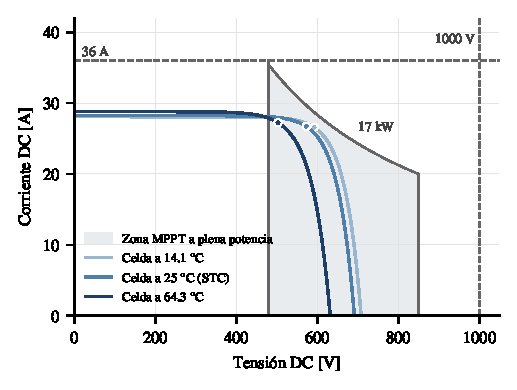
\includegraphics[width=0.92\anchofig]{soa.pdf}
\caption{Área de operación segura de un MPPT con dos cadenas de 17 módulos y curvas I--V aproximadas a \SI{1000}{W/m^2}. Los puntos marcan la máxima potencia.}
\label{fig:soa}
\end{figure}

\subsection{Estimación energética esperada}

La Tabla~\ref{tab:produccion} y la Fig.~\ref{fig:produccion} presentan la generación mensual calculada con \eqref{eq:efv} para \SI{168.3}{kWp}, con las HSP sobre el plano a \SI{10}{\degree} y el $PR$ de cada mes. El sistema generaría \SI{219.5}{MWh} al año, el 98.4\,\% del consumo anual, con un rendimiento de
\begin{equation}
\gamma_{fv} = \frac{E_{fv}}{P_{fv}} = \frac{\SI{219524}{kWh}}{\SI{168.3}{kWp}} = \SI{1304}{kWh/kWp}.
\end{equation}
La mayor generación ocurre en marzo y la menor en noviembre. De enero a abril y en setiembre la generación supera el consumo del mes, mientras que en los demás meses es menor. La energía consumida directamente, la depositada y la devuelta por la red se presentan en la Sección~\ref{sec:economia}.

\begin{table}[!t]
\caption{Pérdida por temperatura ($p_T$), factor de rendimiento, generación mensual estimada (\SI{168.3}{kWp}) y consumo}
\label{tab:produccion}
\centering
\footnotesize
\setlength{\tabcolsep}{2.5pt}
\begin{tabular}{l S[table-format=1.2] S[table-format=1.1] S[table-format=1.3] S[table-format=6.0] S[table-format=6.0] S[table-format=3.1]}
\toprule
{Mes} & {HSP} & {$p_T$ [\%]} & {$PR$} & {$E_{fv}$ [kWh]} & {Cons. [kWh]} & {$E_{fv}$/Cons. [\%]} \\
\midrule
Ene & 4.79 & 7.6 & 0.804 & 20092 & 18482 & 108.7 \\
Feb & 5.30 & 7.8 & 0.803 & 20066 & 17626 & 113.8 \\
Mar & 5.35 & 8.0 & 0.802 & 22395 & 18238 & 122.8 \\
Abr & 4.72 & 8.1 & 0.801 & 19094 & 18850 & 101.3 \\
May & 4.13 & 8.0 & 0.801 & 17262 & 19339 & 89.3 \\
Jun & 4.04 & 7.9 & 0.802 & 16378 & 18482 & 88.6 \\
Jul & 3.97 & 7.8 & 0.803 & 16613 & 18972 & 87.6 \\
Ago & 4.21 & 7.8 & 0.803 & 17638 & 19094 & 92.4 \\
Set & 4.51 & 7.8 & 0.803 & 18305 & 18238 & 100.4 \\
Oct & 4.19 & 7.7 & 0.804 & 17558 & 18727 & 93.8 \\
Nov & 3.90 & 7.7 & 0.804 & 15827 & 17993 & 88.0 \\
Dic & 4.36 & 7.7 & 0.804 & 18296 & 18972 & 96.4 \\
\midrule
Total & {--} & {--} & 0.803 & 219524 & 223013 & 98.4 \\
\bottomrule
\end{tabular}
\end{table}

\begin{figure}[!t]
\centering
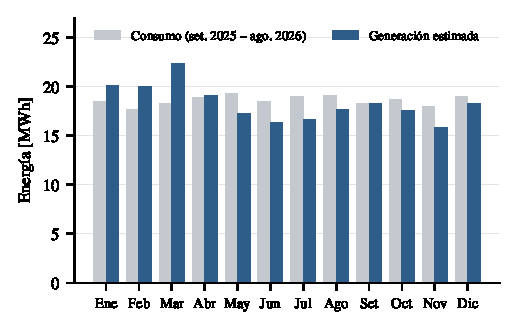
\includegraphics[width=0.92\anchofig]{produccion.pdf}
\caption{Consumo mensual del establecimiento y generación mensual estimada del sistema de \SI{168.3}{kWp}.}
\label{fig:produccion}
\end{figure}

\FloatBarrier
\section{Elementos de instalación}\label{sec:instalacion}

\subsection{Lista de materiales de la estructura de montaje}

Los 374 módulos se distribuyen en 22 filas de este a oeste, con 17 módulos en posición vertical por fila, inclinados \SI{10}{\degree} hacia el sur. Las filas se colocan paralelas al borde corto del techo, por lo que los módulos quedan orientados con un acimut de unos \SI{173}{\degree}, es decir, \SI{7}{\degree} al este del sur (Sección~\ref{sec:lugar}). Con \SI{10}{\degree} de inclinación esta desviación cambia la radiación directa anual sobre los módulos en menos de 0.1\,\%, así que en los cálculos se consideró la orientación sur. Cada fila corresponde a una cadena; las filas se agrupan en dos inversores con cinco cadenas y tres con cuatro, como se muestra en el diagrama unifilar. Cada fila mide unos \SI{19.8}{m}, lo que deja cerca de \SI{0.85}{m} libres a cada lado en el ancho estimado del techo.

La separación entre filas se calculó para que no haya sombra el 21 de diciembre entre las 10:00 y las 14:00 (hora solar):
\begin{equation}
d_1 = \frac{L\,\sin\beta}{\tan h_0} = \frac{\SI{1.757}{m}\cdot\sin\SI{10}{\degree}}{\tan\SI{46.0}{\degree}} = \SI{0.29}{m},
\end{equation}
donde $L$ es el largo del módulo, $\beta$ la inclinación y $h_0$ la altura solar a las 10:00 de ese día (Sección~\ref{sec:recurso}). Sumando la proyección horizontal del módulo, $L\cos\beta=\SI{1.73}{m}$, la distancia mínima entre el inicio de dos filas es de \SI{2.03}{m}. Se adoptaron \SI{2.5}{m}, que dejan un pasillo de mantenimiento. El arreglo ocupa así unos \SI{19.8}{m} $\times$ \SI{54.2}{m} (\SI{1074}{m^2}), el 54\,\% del techo disponible; los módulos suman \SI{745}{m^2}.

Para el montaje se eligió el sistema \textit{SOLARMOUNT} de Unirac \cite{unirac_design}, compatible con el marco de \SI{30}{mm} del módulo. Cada fila lleva dos rieles de aluminio sobre los que se sujetan los módulos con grapas. El riel inferior se apoya directamente en soportes tipo L, mientras que el superior se eleva con patas de inclinación ajustables de 8 a 12 in \cite{unirac_tilt}, que también se fijan con soportes tipo L. Si las patas se dejan en su altura mínima de 8 in (\SI{0.20}{m}), los rieles deben quedar separados unos \SI{1.17}{m} ($\SI{0.20}{m}/\sin\SI{10}{\degree}$) para obtener los \SI{10}{\degree} de inclinación. Al instalar, la altura de las patas y la separación de los rieles se ajustan con las guías de instalación del módulo y de la estructura.

Los soportes se sujetan a la lámina de la cubierta con abrazaderas S-5!, que se escogen según el perfil de la lámina y no requieren perforarla. Cada línea de riel se arma con tres rieles de \SI{6.1}{m} y uno de \SI{3.4}{m}, y la cantidad de soportes se estimó con uno cada \SI{1.2}{m}, es decir, 18 por línea. Con esto se obtuvo la lista de materiales de la Tabla~\ref{tab:montaje}. Los módulos pesan en total unos \SI{8040}{kg}, por lo que todavía falta verificar que la cubierta soporte esta carga y definir la separación final de los soportes según el viento.

\begin{table}[!htb]
\caption{Lista de materiales de la estructura de montaje (22 filas de 17 módulos)}
\label{tab:montaje}
\centering
\footnotesize
\setlength{\tabcolsep}{3pt}
\begin{tabular}{l l r}
\toprule
Elemento & Referencia & Cant. \\
\midrule
Riel de aluminio de \SI{6.1}{m} & Unirac \textit{SM Rail} 240" & 132 \\
Riel de aluminio de \SI{3.4}{m} & Unirac \textit{SM Rail} 132" & 44 \\
Empalme de riel & Unirac \textit{SM Splice} & 132 \\
Grapa intermedia con unión a tierra & Unirac \textit{SM BND Midclamp} & 704 \\
Grapa de extremo & Unirac \textit{SM Endclamp} & 88 \\
Soporte tipo L (rieles y patas) & Unirac \textit{L-Foot} & 792 \\
Pata de inclinación 8--12 in & Unirac 307107M & 396 \\
Fijación a lámina metálica & S-5! (según perfil) & 792 \\
Terminal de tierra para riel & ILSCO \textit{Lay-in Lug} & 44 \\
Conductor de tierra desnudo & Cu 10 AWG & \SI{550}{m} \\
\bottomrule
\end{tabular}
\end{table}

\subsection{Dimensionamiento del cableado en los distintos tramos}

El cableado se dividió en los cuatro tramos de la Tabla~\ref{tab:cables}. Sus longitudes son estimadas, suponiendo que los inversores se ubican junto al cuarto eléctrico. La corriente de diseño se calculó como $i_w=1.25\cdot1.25\cdot I_{sc}$ en el lado DC y como $i_w=1.25\cdot I_{\max}$ en el lado AC. La capacidad de cada conductor se tomó de la Tabla 310.15(B)(16) del NEC 2014, la edición del Código Eléctrico oficializada en Costa Rica \cite{codigo_electrico, nec2014}, y se corrigió por temperatura ambiente (Tabla 310.15(B)(2)(a)) y por agrupamiento (Tabla 310.15(B)(3)(a)). Además, se verificó que la caída de tensión de cada tramo fuera menor a 1.5\,\%, con
\begin{equation}
\Delta V_{\mathrm{DC}} = 2\,L\,I\,R, \qquad \Delta V_{\mathrm{AC}} = \sqrt{3}\,L\,I\,R,
\end{equation}
donde $L$ es la longitud del tramo, $I$ la corriente y $R$ la resistencia del conductor por unidad de longitud \cite{nec2014}.

Entre módulos (tramo 1) se usan los cables de \SI{4}{mm^2} (12 AWG) con conectores MC4 que trae el propio módulo \cite{aiko_ds}.

Para el tramo 2, que va de las cadenas al inversor, la corriente de diseño es $i_w=1.25\cdot1.25\cdot\SI{14.40}{A}=\SI{22.5}{A}$, y se usa \textit{PV Wire} de 10 AWG, que admite \SI{40}{A} a \SI{90}{\celsius}. Las cadenas de cada inversor se llevan en dos canalizaciones de 2 o 3 cadenas, es decir, con 4 a 6 conductores con corriente, lo que reduce la capacidad al 80\,\%. Como en el techo la temperatura ambiente puede llegar a \SI{50}{\celsius} (factor 0.82), la capacidad final es de \SI{26.2}{A}, mayor que $i_w$.

En el tramo 3, del inversor al tablero FV, la corriente nominal de salida es $\SI{25}{kW}/(\sqrt{3}\cdot\SI{208}{V})=\SI{69.4}{A}$, y la ficha da un máximo de \SI{69.5}{A}. Con este valor, la corriente de diseño es $i_w=1.25\cdot\SI{69.5}{A}=\SI{86.9}{A}$. Se usa THHN de 3 AWG, que admite \SI{100}{A} a \SI{75}{\celsius}, o \SI{94}{A} con el factor 0.94 para un ambiente de hasta \SI{35}{\celsius}.

Por último, en el tramo 4, del tablero FV al tablero principal, la corriente de diseño es $i_w=1.25\cdot5\cdot\SI{69.5}{A}=\SI{434.4}{A}$. Se usan dos conductores THHN de 250 kcmil por fase, en canalizaciones separadas. Cada uno admite \SI{255}{A} a \SI{75}{\celsius}, y con el factor 0.94 suman \SI{479}{A}.

\begin{table}[!htb]
\caption{Conductores por tramo}
\label{tab:cables}
\centering
\footnotesize
\setlength{\tabcolsep}{2.5pt}
\begin{tabular}{c c c c c c}
\toprule
Tramo & $L$ [m] & $i_w$ [A] & Conductor & Tierra & $\Delta V$ [\%] \\
\midrule
1 & {--} & {--} & 12 AWG (módulo) & {--} & {--} \\
2 & 40 & 22.5 & 2$\times$10 AWG PV & 10 AWG & 0.86 \\
3 & 15 & 86.9 & 3$\times$3 AWG THHN & 8 AWG & 0.70 \\
4 & 15 & 434.4 & 2$\times$(3$\times$250 kcmil) & 2$\times$2 AWG & 0.37 \\
\bottomrule
\end{tabular}
\\[2pt]
{\footnotesize $L$: longitud estimada en un sentido (tramo 2: cadena más lejana). $\Delta V$ del tramo 2 con $I_{mp}$ y $V_{mp}$ a \SI{64.3}{\celsius}; tramos 3 y 4 con la corriente máxima de salida.}
\end{table}

La caída de tensión es de 0.86\,\% en el lado DC y de 1.06\,\% en el lado AC, sumando los tramos 3 y 4. Los dos valores quedan por debajo del 1.5\,\%. El calibre de los conductores de tierra se eligió según la protección de cada tramo, con la Tabla 250.122 del NEC \cite{nec2014}.

\subsection{Lista de protecciones eléctricas}

En el lado DC, la caja de conexiones de cada inversor ya incluye fusibles para cada entrada, un seccionador DC que puede abrirse con carga y descargadores de sobretensión tipo II \cite{cps_ds}. El fusible de cada cadena debe ser de al menos $1.25\cdot1.25\cdot I_{sc}=1.56\cdot\SI{14.12}{A}=\SI{22.1}{A}$, con la $I_{sc}$ del módulo en STC \cite{nec2014}, y no puede superar los \SI{25}{A} que el módulo admite como fusible máximo en serie \cite{aiko_ds}. Por eso se eligió un fusible gPV de \SI{25}{A} y \SI{1000}{V}. Su tensión supera los \SI{708}{V} de la cadena en frío, y su corriente es menor que la capacidad corregida del conductor de 10 AWG (\SI{26.2}{A}), de modo que el conductor queda protegido. Además, como son inversores sin transformador, incluyen detección de fallas de aislamiento y de corriente a tierra en el lado DC, que el NEC exige en este tipo de arreglos \cite{nec2014}.

En el lado AC, la salida de cada inversor llega al tablero FV a través de un interruptor termomagnético tripolar de \SI{90}{A}. Este valor es mayor que la corriente de diseño de \SI{86.9}{A} y menor que la capacidad corregida del conductor de 3 AWG (\SI{94}{A}) y que la protección máxima que admite el inversor (\SI{125}{A}). Después del termomagnético se coloca un interruptor diferencial tripolar de \SI{100}{A} y \SI{300}{mA}, que protege contra contactos indirectos. El tablero FV tiene además un descargador de sobretensión tipo 2.

Entre el tablero FV y el tablero principal se instala un seccionador visible con bloqueo, que permite aislar el sistema durante trabajos en la red. Es de \SI{600}{A}, el tamaño comercial inmediato superior a la corriente del tramo~4. El sistema se conecta al tablero principal con un interruptor tripolar de \SI{450}{A}, que es el punto de interconexión. Este valor es mayor que la corriente de diseño de \SI{434.4}{A} y menor que la capacidad corregida de los conductores (\SI{479}{A}).

Las barras del tablero principal también deben soportar la corriente que aporta el sistema. Según la regla del 120\,\% del NEC (art.\ 705.12), la suma de la protección principal del tablero y la del sistema no debe superar 1.2 veces la capacidad de las barras \cite{nec2014}. Como no se conocen la capacidad de las barras ni la protección principal, esta comprobación queda pendiente. Si las barras no la cumplen, se podría conectar el sistema antes del interruptor principal del tablero, del lado de la alimentación.

Por último, los marcos, rieles, inversores y tableros se unen al sistema de puesta a tierra del edificio. La Tabla~\ref{tab:protecciones} resume las protecciones.

\begin{table}[!htb]
\caption{Lista de protecciones eléctricas}
\label{tab:protecciones}
\centering
\footnotesize
\setlength{\tabcolsep}{3pt}
\begin{tabular}{l l c}
\toprule
Protección & Características & Cant. \\
\midrule
\multicolumn{3}{l}{\textit{Lado DC (integradas en el inversor)}} \\
Fusible de cadena & gPV, \SI{25}{A}, \SI{1000}{V} DC & 22 \\
Seccionador DC bajo carga & \SI{1000}{V} & 5 \\
DPS DC & Tipo II & 5 \\
\multicolumn{3}{l}{\textit{Lado AC}} \\
Interruptor termomagnético & 3P, \SI{90}{A}, \SI{240}{V} & 5 \\
Interruptor diferencial & 3P, \SI{100}{A}, \SI{300}{mA} & 5 \\
DPS AC & Tipo 2, \SI{240}{V} & 1 \\
Seccionador visible con bloqueo & 3P, \SI{600}{A}, \SI{600}{V} & 1 \\
Interruptor de interconexión & 3P, \SI{450}{A}, \SI{240}{V} & 1 \\
\multicolumn{3}{l}{\textit{Puesta a tierra}} \\
Unión de marcos y rieles & Grapas BND y terminales & -- \\
Barra de tierra & A electrodos del edificio & 1 \\
\bottomrule
\end{tabular}
\end{table}

\FloatBarrier
\subsection{Diagrama unifilar detallado}

La Fig.~\ref{fig:unifilar} presenta el diagrama unifilar de la instalación, dibujado con la simbología normalizada IEC 60617. En él se muestran las 22 cadenas de 17 módulos, su conexión a cada MPPT de los cinco inversores, las protecciones de los lados DC y AC, los conductores de cada tramo y la conexión, mediante el interruptor de \SI{450}{A}, al tablero principal y al medidor bidireccional del ICE. El diagrama incluye además una leyenda de símbolos, un resumen de los conductores y las especificaciones principales del sistema.

\begin{figure*}[p]
\centering
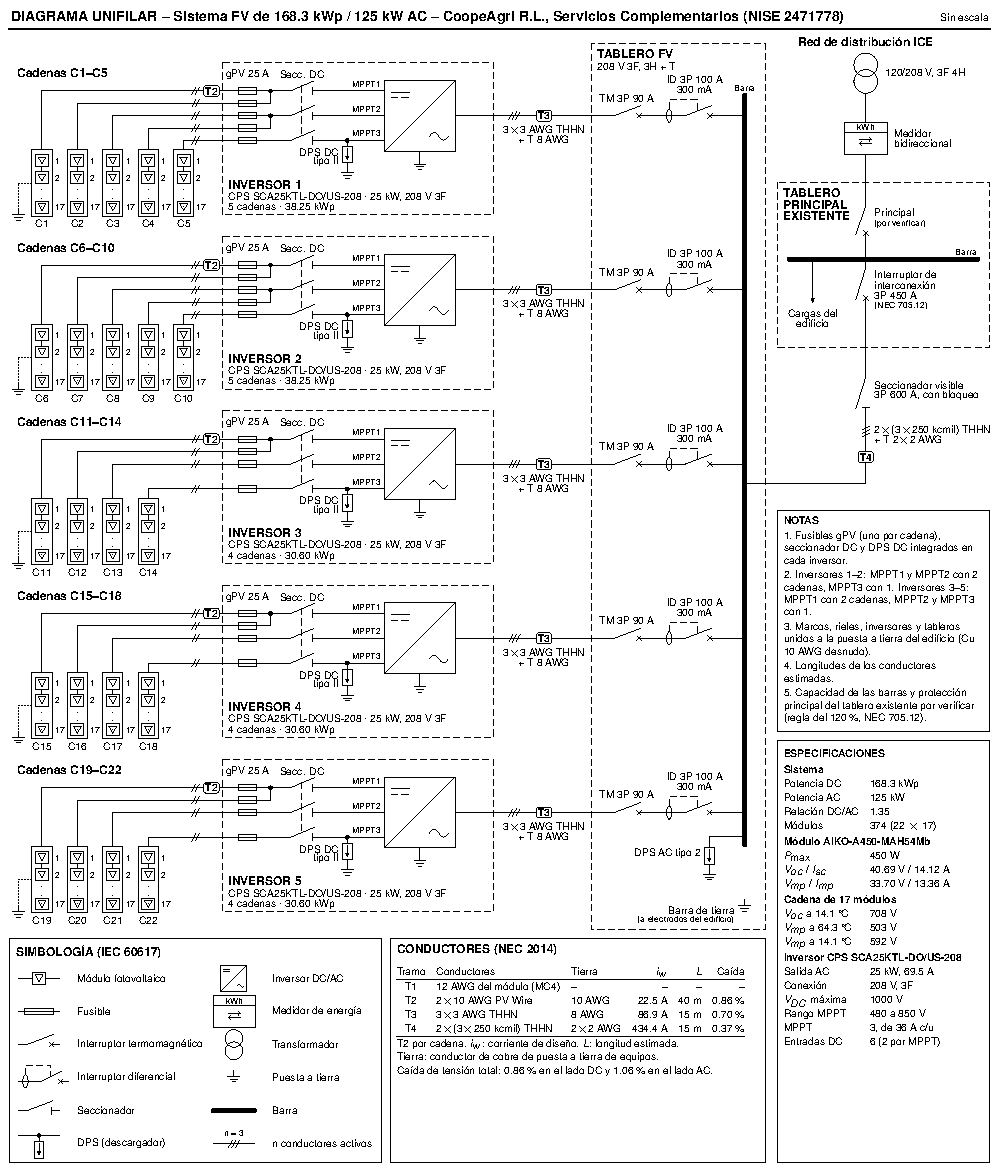
\includegraphics[width=\textwidth]{unifilar.pdf}
\caption{Diagrama unifilar del sistema fotovoltaico propuesto (\SI{168.3}{kWp} / \SI{125}{kW} AC), con simbología IEC 60617.}
\label{fig:unifilar}
\end{figure*}

\section{Estimación económica del retorno}\label{sec:economia}

Para evaluar el retorno se estimaron el costo del sistema, la factura con y sin el sistema y el flujo de caja a 25 años. Los montos se expresan en colones con un tipo de cambio de ¢456.61 por dólar \cite{tipo_cambio}.

\subsection{Costo del sistema}

El costo inicial incluye los módulos, los inversores, la estructura, los conductores, las protecciones, los trámites y la instalación (Tabla~\ref{tab:costos}). Los equipos se valoraron con precios de lista de tiendas de Estados Unidos y Europa de octubre de 2026 \cite{precio_modulo, precio_inversor, precios_bos}. Los tableros, las canalizaciones, los interruptores diferenciales y los accesorios de puesta a tierra se estimaron como un 15\,\% de los conductores y protecciones. Los servicios se estimaron de la siguiente forma:
\begin{itemize}
\item \textbf{Diseño:} honorarios mínimos del arancel del CFIA, 0.5\,\% por estudios preliminares y 4\,\% por planos y especificaciones, aplicados al valor de la obra (equipos e instalación, ¢94.3 millones) \cite{cfia_arancel}. El arancel está escrito para edificaciones, por lo que su uso en un sistema fotovoltaico es una aproximación.
\item \textbf{Registro del proyecto ante el CFIA:} derecho de asistencia técnica (0.15\,\%) y timbre (0.10\,\%) sobre el valor de la obra \cite{cfia_registro, cfia_resumen}.
\item \textbf{Interconexión con el ICE:} cargos de las cuatro etapas aprobados para 2026 \cite{ice_der}. La revisión de disponibilidad de potencia del circuito forma parte de la primera etapa \cite{ice_guia2021}, y por eso no se agregó un cobro aparte por viabilidad.
\item \textbf{Instalación y ganancia del instalador:} no se encontraron valores públicos para Costa Rica, así que se supusieron ¢\num{100000} por kWp para la mano de obra y un 20\,\% de ganancia sobre el costo total.
\end{itemize}
Para comprobar que estos supuestos son razonables se hicieron dos comparaciones. La primera es con el estudio de costos de NREL para sistemas comerciales en techo \cite{nrel_benchmark}. Si se aplican sus horas de trabajo, salarios, gastos generales, contingencia y utilidad a los equipos de la Tabla~\ref{tab:costos}, sin los gastos del desarrollador propios del mercado de Estados Unidos, la mano de obra, los gastos generales y la utilidad suman USD 0.47 por watt, frente a USD 0.48 por watt con los supuestos usados. Como los salarios en Costa Rica son menores que los de Estados Unidos, el costo de mano de obra supuesto probablemente es alto. La segunda comparación es con los precios publicados por un instalador nacional para sistemas comerciales e industriales, de ¢0.75 a ¢0.80 millones por kW con diseño y trámites incluidos \cite{sunshine_precios}. El precio resultante, de ¢0.71 millones por kWp (USD 1.55 por watt), queda por debajo de ese intervalo; por eso se incluye una sensibilidad con un precio 15\,\% mayor (Tabla~\ref{tab:sensibilidad}).

El costo real puede ser mayor, porque no se incluyeron el flete, la nacionalización y el IVA de los equipos, ni equipos especiales, como grúas, para subir los materiales al techo. Tampoco se incluyeron dispositivos de apagado rápido en cada módulo; el inversor seleccionado solo trae la caja de conexiones preparada para ese apagado, y podrían necesitarse si el ICE o el inspector los exigen según el NEC (art.\ 690.12) \cite{nec2014}. Antes de construir, el precio debe confirmarse con cotizaciones formales.

\begin{table}[!htb]
\caption{Costo estimado del sistema de \SI{168.3}{kWp}}
\label{tab:costos}
\centering
\footnotesize
\setlength{\tabcolsep}{4pt}
\begin{tabular}{l S[table-format=6.0]}
\toprule
{Rubro} & {Monto [USD]} \\
\midrule
Módulos (374 $\times$ \SI{148.03}{USD}) & 55364 \\
Inversores (5 $\times$ \SI{8997.44}{USD}) & 44987 \\
Estructura de montaje (Tabla~\ref{tab:montaje}) & 43010 \\
Conductores & 7927 \\
Protecciones (Tabla~\ref{tab:protecciones}) & 15022 \\
Otros materiales eléctricos (15\,\%) & 3442 \\
\midrule
Subtotal de equipos & 169752 \\
\midrule
Diseño, honorarios CFIA (4.5\,\%) & 9297 \\
Registro ante el CFIA (0.25\,\%) & 517 \\
Interconexión ICE, etapas 1--4 (¢\num{382871}) & 839 \\
Instalación (¢\num{16830000}) & 36859 \\
\midrule
Costo total & 217264 \\
Ganancia del instalador (20\,\%) & 43453 \\
\midrule
\textbf{Precio del sistema} & 260717 \\
\bottomrule
\end{tabular}
\\[2pt]
{\footnotesize Equivale a ¢119.05 millones, o \SI{1.55}{USD} por watt instalado.}
\end{table}

\subsection{Balance de energía}

La Tabla~\ref{tab:balance} presenta el balance mensual con medición neta sencilla, según las reglas y el perfil de carga descritos en la Sección~\ref{sec:red}. El edificio consume directamente \SI{112.5}{MWh} al año, el 51.2\,\% de la generación. De los \SI{107.1}{MWh} depositados se reconocen \SI{103.0}{MWh}; los \SI{4.0}{MWh} restantes corresponden a los meses secos, cuando el depósito supera el 49\,\%. Toda la energía reconocida se devuelve dentro del año: en los meses de mayor generación se acumula un saldo que se usa en los meses siguientes. Con esto, la energía comprada a la red baja de 223.0 a \SI{7.5}{MWh} al año.

\begin{table}[!htb]
\caption{Balance mensual de energía con medición neta y ahorro anual (sin degradación)}
\label{tab:balance}
\centering
\footnotesize
\setlength{\tabcolsep}{1.1pt}
\begin{tabular}{l S[table-format=6.0] S[table-format=6.0] S[table-format=6.0] S[table-format=6.0] S[table-format=6.0] S[table-format=4.0] S[table-format=5.0]}
\toprule
{Mes} & {Gen.} & {Autoc.} & {Dep.} & {Rec.} & {Dev.} & {Compra} & {Ahorro} \\
 & {[kWh]} & {[kWh]} & {[kWh]} & {[kWh]} & {[kWh]} & {[kWh]} & {[miles ¢]} \\
\midrule
Ene & 20092 & 9174 & 10918 & 9845 & 9308 & 0 & 1248 \\
Feb & 20066 & 9394 & 10672 & 9832 & 8232 & 0 & 1188 \\
Mar & 22395 & 9788 & 12607 & 10974 & 8450 & 0 & 1230 \\
Abr & 19094 & 9457 & 9637 & 9356 & 9393 & 0 & 1273 \\
May & 17262 & 9617 & 7645 & 7645 & 9722 & 0 & 1308 \\
Jun & 16378 & 9177 & 7201 & 7201 & 9305 & 0 & 1248 \\
Jul & 16613 & 9230 & 7383 & 7383 & 7826 & 1916 & 1148 \\
Ago & 17638 & 9628 & 8010 & 8010 & 8010 & 1456 & 1188 \\
Set & 18305 & 9958 & 8347 & 8347 & 8280 & 0 & 1230 \\
Oct & 17558 & 9343 & 8215 & 8215 & 8282 & 1102 & 1187 \\
Nov & 15827 & 8577 & 7250 & 7250 & 7250 & 2166 & 1061 \\
Dic & 18296 & 9109 & 9187 & 8965 & 8965 & 898 & 1219 \\
\midrule
Total & 219524 & 112452 & 107072 & 103023 & 103023 & 7538 & 14528 \\
\bottomrule
\end{tabular}
\\[2pt]
\parbox{\columnwidth}{\footnotesize Gen.: generación de la Tabla~\ref{tab:produccion}. Autoc.: consumida en el edificio, según el balance horario. Dep.: depositada en la red. Rec.: depositada reconocida (máximo 49\,\% de Gen.). Dev.: devuelta por la red, incluido el saldo de meses anteriores. Compra: energía comprada a la red.}
\end{table}

\subsection{Facturación con y sin el sistema}

La factura sin el sistema se calculó con los cargos T-CO de 2026 \cite{ice_facturas}: \SI{59.67}{¢/kWh} de energía, ¢\num{9861.68} por kW de demanda, \SI{2.70}{¢/kWh} de alumbrado público, IVA del 13\,\% sobre energía y demanda, y ¢\num{1827.40} del tributo de bomberos. Con estos cargos el modelo reproduce los montos facturados de enero a agosto de 2026. El total anual con los cargos de 2026 es de ¢21.88 millones, de los cuales ¢6.22 millones corresponden a la demanda; es menor que lo facturado en el período (¢23.15 millones) porque los meses de 2025 tenían cargos más altos.

Con el sistema:
\begin{itemize}
\item la energía comprada paga los mismos cargos de energía y alumbrado, y la energía devuelta por la red no se cobra;
\item no se aplica tarifa de acceso, porque la metodología vigente la establece solo para clientes con tarifa monómica, y la T-CO es binómica (cobra energía y demanda) \cite{aresep_metodologia};
\item se agrega la tarifa TDER, con la que la distribuidora recupera los costos de integrar la generación distribuida a su red, de ¢255 por kW instalado al mes más IVA \cite{ice_der}; se aplicó a los \SI{168.3}{kWp} del arreglo (¢\num{582000} al año), lo que es conservador, porque si se aplica a los \SI{125}{kW} de los inversores el cargo es menor;
\item en el caso base la demanda facturada se mantiene igual.
\end{itemize}
La conexión requiere que el circuito y el transformador del ICE tengan capacidad para la potencia del sistema, condición que el ICE revisa al estudiar la solicitud \cite{ice_guia}.

Con estas condiciones la factura anual baja de ¢21.88 a ¢7.36 millones, un ahorro de ¢14.53 millones (66.4\,\%) sin considerar la degradación de los módulos (Fig.~\ref{fig:facturacion}). Lo que queda de la factura corresponde sobre todo al cargo por demanda, que no cambia, y a la tarifa TDER.

\begin{figure}[!htb]
\centering
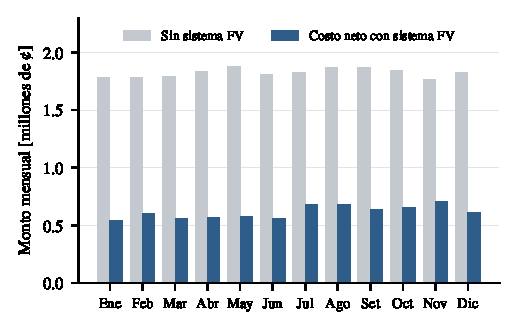
\includegraphics[width=\anchofig]{facturacion.pdf}
\caption{Factura mensual sin el sistema y con el sistema, con cargos de 2026.}
\label{fig:facturacion}
\end{figure}

\subsection{Flujo de caja e indicadores}

El flujo de caja se proyectó con los supuestos de la Tabla~\ref{tab:supuestos}, para el pago de contado y para el caso en que se financia el 80\,\% con un préstamo. La Tabla~\ref{tab:indicadores} presenta el valor presente neto (VPN), la tasa interna de retorno (TIR), el índice de rentabilidad (IR, valor presente de los flujos entre la inversión) y el período de recuperación (PRI).

La tasa de descuento de 7\,\% es un supuesto que representa el costo de oportunidad del dinero para la cooperativa: es mayor que la tasa básica pasiva, de 3.59\,\% en setiembre de 2026 \cite{bccr_tbp}, y similar a la tasa activa promedio de los créditos en colones para comercio, de 6.6\,\% \cite{bccr_tan}. Para el préstamo se supuso un interés de 9\,\%, entre las tasas activas para comercio (6.6\,\%) y para servicios (11.7\,\%) \cite{bccr_tan}, a 120 meses y con el 80\,\% financiado, condiciones similares a las ofrecidas para financiar paneles solares en el país \cite{bancopopular, avolta}.

\begin{table}[!htb]
\caption{Supuestos del flujo de caja}
\label{tab:supuestos}
\centering
\footnotesize
\setlength{\tabcolsep}{3pt}
\begin{tabular}{l l}
\toprule
Parámetro & Valor \\
\midrule
Horizonte / tasa de descuento & 25 años / 7\,\% \\
Aumento anual de tarifas y gastos & 0\,\% (base) y 3\,\% \\
Degradación (solo energía) & 1\,\% (año 1); 0.35\,\%/año \\
Mantenimiento y reposición & 1\,\% del precio por año \\
Préstamo & 80\,\% a 9\,\% anual, 120 cuotas \\
Cuota mensual del préstamo & ¢\num{1206419} \\
\bottomrule
\end{tabular}
\end{table}

\begin{table}[!htb]
\caption{Indicadores económicos (25 años)}
\label{tab:indicadores}
\centering
\footnotesize
\setlength{\tabcolsep}{3pt}
\begin{tabular}{l c S[table-format=2.1] S[table-format=2.1] S[table-format=1.2] S[table-format=2.1]}
\toprule
{Pago} & {Aumento} & {VPN} & {TIR} & {IR} & {PRI} \\
 & {anual} & {[M¢]} & {[\%]} & & {[años]} \\
\midrule
Contado (proyecto) & 0\,\% & 29.5 & 9.7 & 1.25 & 9.2 \\
Contado (proyecto) & 3\,\% & 75.6 & 12.6 & 1.63 & 8.2 \\
Préstamo (aporte propio) & 0\,\% & 23.0 & 10.7 & 1.97 & 13.1 \\
Préstamo (aporte propio) & 3\,\% & 69.1 & 16.0 & 3.90 & 11.2 \\
\bottomrule
\end{tabular}
\\[2pt]
{\footnotesize Con préstamo, la inversión inicial de los propietarios es de ¢23.81 millones. Los indicadores del proyecto y los del aporte propio tienen bases distintas y no se comparan entre sí.}
\end{table}

En el flujo de caja, la degradación del 1\,\% se aplica desde el primer año y el ahorro del año 1 queda en ¢14.38 millones; al restar el mantenimiento, el flujo neto es de ¢13.19 millones. En el caso base, pagando de contado, la inversión se recupera en 9.2 años, la TIR (9.7\,\%) supera la tasa de descuento y cada colón invertido devuelve 1.25 colones en valor presente. Con préstamo, la cuota anual (¢14.48 millones) es mayor que el flujo neto, por lo que durante los diez años del crédito el flujo es negativo, de unos ¢1.3 millones por año y la recuperación se extiende a 13.1 años (Fig.~\ref{fig:flujo}); este plazo se mide sobre el aporte propio de ¢23.81 millones y no sobre el precio total del sistema.

\begin{figure}[!htb]
\centering
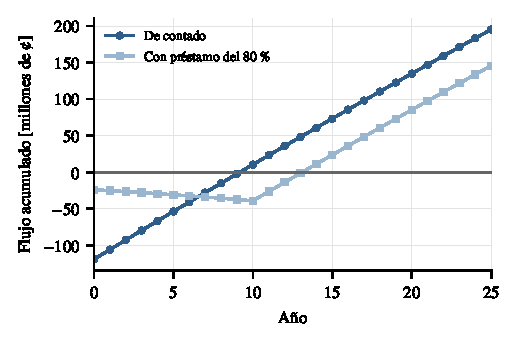
\includegraphics[width=\anchofig]{flujo_acumulado.pdf}
\caption{Flujo de caja acumulado sin aumento de tarifas.}
\label{fig:flujo}
\end{figure}

La Tabla~\ref{tab:sensibilidad} muestra cómo cambian los resultados de contado al variar los supuestos con mayor incertidumbre. Los escenarios que más cambian el resultado son los de los excedentes: como cerca de la mitad de la generación se deposita en la red, el VPN se vuelve negativo si esa energía se vende a \SI{27.40}{¢/kWh} o no se reconoce. Como escenario hipotético también se evaluó una tarifa de acceso de \SI{25}{¢/kWh} sobre la energía devuelta, que hoy no aplica a la T-CO; con ella el VPN bajaría a ¢3.7 millones. En cuanto al perfil de carga, con una carga diurna del 50\,\% de la demanda el autoconsumo baja al 41\,\% de la generación. Como la energía que deja de consumirse se deposita en la red, el ahorro disminuye solo un 9\,\%, pero el VPN se reduce a la mitad (¢14.6 millones). Por último, la tasa de descuento y el precio del sistema son supuestos sin fuente pública: con una tasa de 9\,\% o un precio 15\,\% mayor, el VPN baja a ¢6.5 y ¢9.5 millones, aunque sigue positivo.

La reducción de la demanda facturada se presenta solo como sensibilidad, porque ocurriría únicamente si la generación coincide con el intervalo en que se registra el máximo del mes, lo que no puede comprobarse sin mediciones horarias.

\begin{table}[!htb]
\caption{Sensibilidad de los resultados (contado, sin aumento de tarifas)}
\label{tab:sensibilidad}
\centering
\footnotesize
\setlength{\tabcolsep}{3pt}
\begin{tabular}{l S[table-format=2.2] S[table-format=-2.1] S[table-format=2.1] S[table-format=2.1]}
\toprule
{Escenario} & {Ahorro} & {VPN} & {TIR} & {PRI} \\
 & {[M¢]} & {[M¢]} & {[\%]} & {[años]} \\
\midrule
Caso base (medición neta) & 14.53 & 29.5 & 9.7 & 9.2 \\
Demanda facturada $-10$\,\% & 15.15 & 36.7 & 10.3 & 8.7 \\
Demanda facturada $-20$\,\% & 15.77 & 44.0 & 10.9 & 8.4 \\
Neteo con tarifa de acceso & 12.20 & 3.7 & 7.3 & 11.2 \\
Venta de excedentes & 10.24 & -18.6 & 5.2 & 13.7 \\
Excedentes sin reconocimiento & 7.89 & -44.6 & 2.3 & 18.7 \\
Carga diurna: 50\,\% de $D$ & 13.20 & 14.6 & 8.4 & 10.2 \\
Carga diurna: 65\,\% de $D$ & 14.21 & 25.9 & 9.4 & 9.4 \\
Carga diurna: 85\,\% de $D$ & 14.72 & 31.6 & 9.9 & 9.0 \\
Tasa de descuento 5\,\% & 14.53 & 59.9 & 9.7 & 9.2 \\
Tasa de descuento 9\,\% & 14.53 & 6.5 & 9.7 & 9.2 \\
Precio del sistema $+15$\,\% & 14.53 & 9.5 & 7.8 & 10.7 \\
\bottomrule
\end{tabular}
\\[2pt]
{\footnotesize $D$: demanda facturada del mes. Caso base: 75\,\% de $D$.}
\end{table}

\subsection{Comparación con otras potencias}\label{sec:alternativas}

Para conocer cómo cambia la rentabilidad con el tamaño, la Tabla~\ref{tab:alternativas} compara el sistema seleccionado con sistemas de menor potencia, formados con cadenas completas de 17 módulos y evaluados con el mismo modelo.

\begin{table*}[!htb]
\caption{Comparación de potencias (año 1, medición neta sencilla)}
\label{tab:alternativas}
\centering
\footnotesize
\setlength{\tabcolsep}{5pt}
\begin{tabular}{S[table-format=3.1] c c S[table-format=1.2] S[table-format=3.1] S[table-format=2.1] S[table-format=2.1] S[table-format=2.2] S[table-format=2.1] S[table-format=2.1] S[table-format=2.1]}
\toprule
{$P_{fv}$} & {Cadenas} & {Inversores} & {DC/AC} & {Inversión} & {Gen./Cons.} & {Depositada} & {Ahorro} & {VPN} & {TIR} & {PRI} \\
{[kWp]} & & {(kW AC)} & & {[M¢]} & {[\%]} & {[\% Gen.]} & {[M¢]} & {[M¢]} & {[\%]} & {[años]} \\
\midrule
76.5 & $10\times17$ & 2 (50 kW) & 1.53 & 52.5 & 44.7 & 12.6 & 6.72 & 16.5 & 10.4 & 8.7 \\
107.1 & $14\times17$ & 3 (75 kW) & 1.43 & 74.7 & 62.6 & 27.9 & 9.42 & 21.9 & 10.2 & 8.8 \\
137.7 & $18\times17$ & 4 (100 kW) & 1.38 & 95.9 & 80.5 & 39.9 & 12.12 & 28.3 & 10.2 & 8.8 \\
153.0 & $20\times17$ & 4 (100 kW) & 1.53 & 103.2 & 89.3 & 44.6 & 13.38 & 34.4 & 10.6 & 8.6 \\
168.3 & $22\times17$ & 5 (125 kW) & 1.35 & 119.0 & 98.4 & 48.8 & 14.53 & 29.5 & 9.7 & 9.2 \\
\bottomrule
\end{tabular}
\\[2pt]
{\footnotesize Gen./Cons.: generación anual respecto al consumo (\SI{223.0}{MWh}). Depositada: energía entregada a la red respecto a la generación. Ahorro del año 1 sin degradación. VPN a 25 años con tasa de 7\,\%, pago de contado y sin aumento de tarifas. Para 107.1, 137.7 y \SI{153}{kWp}, el alimentador y sus protecciones se estimaron por escalamiento.}
\end{table*}

Con la medición neta, el ahorro crece casi en proporción a la potencia, porque la energía depositada se recupera más adelante. Todas las alternativas tienen un VPN positivo y una TIR cercana al 10\,\%. El sistema de \SI{153}{kWp} tiene el VPN más alto, porque el de \SI{168.3}{kWp} necesita un quinto inversor y protecciones de mayor capacidad para un 10\,\% más de generación; la diferencia es de ¢4.9 millones de VPN y 0.9 puntos de TIR, y se mantuvo la propuesta de \SI{168.3}{kWp} porque su generación anual se acerca más al consumo del establecimiento.

\section{Conclusiones}

Con 374 módulos se obtiene una potencia instalada de \SI{168.3}{kWp} y una generación estimada equivalente al 98.4\,\% del consumo anual del edificio. El arreglo ocupa cerca del 54\,\% del techo considerado, así que hay espacio para la distribución propuesta. Las 22 cadenas de 17 módulos se mantienen dentro de los límites eléctricos de los inversores en las temperaturas evaluadas.

Para la acometida de 120/\SI{208}{V} se seleccionaron cinco inversores de \SI{25}{kW} fabricados para esa tensión. El quinto inversor encarece el sistema: la alternativa de \SI{153}{kWp}, con cuatro inversores, tiene un VPN de ¢34.4 millones frente a ¢29.5 millones del sistema seleccionado, aunque su generación cubre solo el 89.3\,\% del consumo.

Con el perfil de consumo supuesto, la energía comprada a la red disminuiría cerca de un 97\,\%. La factura, en cambio, se reduciría un 66.4\,\%, principalmente porque el cargo por demanda se mantiene y se agrega la tarifa TDER. Para saber si el sistema también reduciría la demanda facturada se necesitan mediciones horarias del consumo.

Con el precio estimado y el pago de contado, la inversión se recuperaría en 9.2 años, con una TIR de 9.7\,\%, mayor que la tasa de descuento de 7\,\%. Si se financia el 80\,\% a diez años, la cuota sería mayor que el ahorro neto durante el plazo del préstamo, en unos ¢1.3 millones por año. La cooperativa tendría que cubrir esa diferencia hasta terminar de pagarlo.

La rentabilidad depende de que se mantengan las condiciones actuales de la medición neta sencilla, porque cerca de la mitad de la generación estimada se deposita en la red. Si esa energía se vendiera como excedente o no se reconociera, el VPN sería negativo. Antes de tomar una decisión de inversión deben confirmarse las condiciones de medición neta con el ICE, el precio mediante cotizaciones, la capacidad estructural del techo y las condiciones de conexión tanto en el tablero principal como en la red de distribución.


\section*{Herramientas de apoyo}

Durante el proyecto se utilizó inteligencia artificial para revisar partes de la redacción y ayudar a preparar algunas gráficas, diagramas y scripts de cálculo. Antes de incluir los resultados en el informe, fueron revisados con los datos del sitio y las especificaciones de los equipos. La configuración propuesta y las conclusiones fueron decisiones del grupo.

\begin{thebibliography}{99}
\bibitem{ice_facturas} Instituto Costarricense de Electricidad, ``Facturas eléctricas del servicio NISE 2471778, COOPEAGRI EL GENERAL R.L., meses de cobro noviembre 2025, abril 2026 y agosto 2026,'' 2025--2026.
\bibitem{nasa_power} NASA Langley Research Center, ``POWER Climatology API v2.10.1, promedios 2001--2025,'' [En línea]. Disponible: \url{https://power.larc.nasa.gov/}. Consultado: 9 oct. 2026.
\bibitem{nasa_power_horario} NASA Langley Research Center, ``POWER Hourly API: ALLSKY\_SFC\_SW\_DWN y T2M (2015--2024) y T2M (2005--2025), hora estándar local,'' [En línea]. Disponible: \url{https://power.larc.nasa.gov/}. Consultado: 10 oct. 2026.
\bibitem{uoregon} University of Oregon Solar Radiation Monitoring Laboratory, ``Sun path chart program,'' [En línea]. Disponible: \url{http://solardata.uoregon.edu/SunChartProgram.php}. Consultado: 9 oct. 2026.
\bibitem{pvgis} European Commission, Joint Research Centre, ``Photovoltaic Geographical Information System (PVGIS) v5.3, base PVGIS-ERA5 2005--2023,'' [En línea]. Disponible: \url{https://re.jrc.ec.europa.eu/pvg_tools/en/}. Consultado: 9 oct. 2026.
\bibitem{imn_castro} V. Castro, ``Radiación solar global en Costa Rica,'' Nota de Investigación N.\textsuperscript{o} 6, Instituto Meteorológico Nacional, Ministerio de Agricultura y Ganadería, San José, Costa Rica, 1987.
\bibitem{nasa_power_diario} NASA Langley Research Center, ``POWER Data Access Viewer: series diarias de ALLSKY\_SFC\_SW\_DWN, ALLSKY\_SFC\_SW\_DNI y ALLSKY\_SFC\_SW\_DIFF, 2025 (CERES SYN1deg Ed.~4.1),'' [En línea]. Disponible: \url{https://power.larc.nasa.gov/data-access-viewer/}. Consultado: 11 oct. 2026.
\bibitem{factores_k} Cleanergysolar, ``Tablas: factor de corrección $K$ para superficies inclinadas,'' [En línea]. Disponible: \url{https://www.cleanergysolar.com}.
\bibitem{aiko_manual} Shenzhen Aiko Digital Energy Technology Co., Ltd., ``PV module installation manual (single glass),'' rev.~1.9, abr. 2024. [En línea]. Disponible: \url{https://aikosolar.com/wp-content/uploads/2024/04/PV-Module-Installation-Manual-Single-Glass-EN.pdf}. Consultado: 27 oct. 2026.
\bibitem{aiko_ds} AIKO, ``Neostar 2S AIKO-A-MAH54Mb, 440--470 W: hoja de datos,'' versión V6.3. [En línea]. Disponible: \url{https://www.solartraders.com/uploads/production/data_sheet/file/37607/data_sheet_aiko_a_mah54mb_glas_folie_neostar_2s_de_01-12-2024.pdf}. Consultado: 9 oct. 2026.
\bibitem{decreto43879} Costa Rica, Decreto Ejecutivo N.\textsuperscript{o} 43879-MINAE, ``Reglamento a la Ley N.\textsuperscript{o} 10086 de promoción y regulación de recursos energéticos distribuidos a partir de fuentes renovables,'' 2023.
\bibitem{cps_ds} CPS Chint Power Systems America, ``SCA25KTL-DO/US-208: 25 kW three-phase string inverter, hoja de datos,'' jul. 2025. [En línea]. Disponible: \url{https://www.solarelectricsupply.com/media/sparsh/product_attachment/CPS-SCA25KTL-DO-US-208-Datasheet-7-30-2025.pdf}. Consultado: 9 oct. 2026.
\bibitem{unirac_design} Unirac, ``U-Builder: herramienta de diseño,'' [En línea]. Disponible: \url{https://design.unirac.com/}. Consultado: 9 oct. 2026.
\bibitem{unirac_tilt} Unirac, ``Adjustable tilt legs,'' [En línea]. Disponible: \url{https://unirac.com/products/attachments/adjustable-tilt-legs/}. Consultado: 9 oct. 2026.
\bibitem{codigo_electrico} Costa Rica, Decreto Ejecutivo N.\textsuperscript{o} 36979-MEIC, ``RTCR 458:2011 Reglamento de oficialización del Código Eléctrico de Costa Rica para la seguridad de la vida y de la propiedad,'' y sus reformas (Decreto 43418-MEIC).
\bibitem{nec2014} National Fire Protection Association, \textit{NFPA 70: National Electrical Code}, ed. 2014. Quincy, MA, EE.\,UU.: NFPA, 2014.
\bibitem{tipo_cambio} Telediario, ``Dólar en Costa Rica: tipo de cambio para este viernes 9 de octubre,'' 9 oct. 2026. [En línea]. Disponible: \url{https://telediario.cr/nacional/dolar-costa-rica-tipo-cambio-viernes-9-octubre}.
\bibitem{precio_modulo} Cambio Energético, ``Panel solar AIKO Neostar 2S 450 W,'' [En línea]. Disponible: \url{https://www.cambioenergetico.com/producto/aiko-neostar-2s-450w/}. Consultado: 9 oct. 2026.
\bibitem{precio_inversor} Solar Cellz USA, ``CPS SCA25KTL-DO/US-208-APS 25 kW 3-phase string inverter with APS RSD wirebox,'' [En línea]. Disponible: \url{https://shop.solarcellzusa.com/products/cps-sca25ktl-do-us-208-aps-25-kw-3-phase-string-inverter-with-aps-rsd-wirebox}. Consultado: 9 oct. 2026.
\bibitem{precios_bos} Precios consultados el 9 y el 11 oct. 2026 en: PES Supply (\url{https://www.portlandiaelectric.supply}): Unirac 303019M y 307107M, S-5-U Mini, PV Wire 10 AWG; Elliott Electric Supply (\url{https://www.elliottelectric.com}): THHN 3 AWG, 3/0 AWG y 250 kcmil; SuperBreakers (\url{https://superbreakers.com}): Square D QDL32090, LAL36175 y MAL36450; SupplyHouse (\url{https://www.supplyhouse.com}): Square D D324N; Standard Electric Supply (\url{https://www.standardelectricsupply.com}): Square D HU366.
\bibitem{cfia_arancel} Costa Rica, Decreto Ejecutivo N.\textsuperscript{o} 18636-MOPT, ``Arancel de servicios profesionales de consultoría para edificaciones,'' \textit{La Gaceta} N.\textsuperscript{o} 225, 25 nov. 1988. [En línea]. Disponible: \url{https://cfia.or.cr/site/wp-content/uploads/2024/pdf/descargas/reglamentos/ejercicio/arancel-de-servicios-profesionales-de-consultoria-para-edificaciones.pdf}. Consultado: 11 oct. 2026.
\bibitem{cfia_registro} Colegio Federado de Ingenieros y de Arquitectos de Costa Rica, ``Registro de responsabilidad por consultorías varias,'' Centro de ayuda CFIA. [En línea]. Disponible: \url{https://centrodeayuda.cfia.or.cr/hc/es/articles/360025821333}. Consultado: 11 oct. 2026.
\bibitem{cfia_resumen} Bitántica, ``Aranceles CFIA 2026: tabla de honorarios profesionales para ingenieros y arquitectos,'' 2026. [En línea]. Disponible: \url{https://bitantica.com/blog/aranceles-cfia-2026-honorarios-profesionales}. Consultado: 11 oct. 2026.
\bibitem{ice_der} Instituto Costarricense de Electricidad, ``Tarifas aplicables a recursos energéticos distribuidos: cargos de interconexión, tarifa de acceso, compra-venta de excedentes 2026 y tarifa TDER,'' actualizado 29 jul. 2026. [En línea]. Disponible: \url{https://www.grupoice.com/wps/wcm/connect/6b387ffa-400d-41dd-85aa-76e36daffb20/TARIFAS_APLICABLES_A_RECURSOS_ENERGETICOS_DISTRIBUIDOS_ENERO_2025.pdf}. Consultado: 10 oct. 2026.
\bibitem{ice_guia2021} Instituto Costarricense de Electricidad, División Distribución y Comercialización, ``Guía para el proceso de solicitud de instalación de sistemas de generación distribuida, modalidad neta sencilla,'' set. 2021. [En línea]. Disponible: \url{https://www.grupoice.com/wps/wcm/connect/4cc0b3e7-fa48-4c7c-ac75-b112d4ae9448/Gui%CC%81a+de+Interconexio%CC%81n+Generacio%CC%81n+Distribuida.pdf}. Consultado: 11 oct. 2026.
\bibitem{nrel_benchmark} V. Ramasamy, J. Zuboy, E. O'Shaughnessy, D. Feldman, J. Desai, M. Woodhouse, P. Basore y R. Margolis, ``U.S. solar photovoltaic system and energy storage cost benchmarks, with minimum sustainable price analysis: Q1 2022,'' National Renewable Energy Laboratory, Golden, CO, EE.\,UU., Rep. técnico NREL/TP-7A40-83586, set. 2022. [En línea]. Disponible: \url{https://docs.nlr.gov/docs/fy22osti/83586.pdf}. Consultado: 27 oct. 2026.
\bibitem{sunshine_precios} Sunshine Tech, ``Precio de paneles solares en Costa Rica'' y ``Paneles solares industriales en Costa Rica,'' 2025. [En línea]. Disponible: \url{https://sunshine.tech/precios/}. Consultado: 11 oct. 2026.
\bibitem{aresep_metodologia} Autoridad Reguladora de los Servicios Públicos, ``RE-0076-JD-2023: Metodología tarifaria derivada de la Ley 10086 (ajustada con RE-0126-JD-2024),'' [En línea]. Disponible: \url{https://www.grupoice.com/wps/wcm/connect/e9837ac4-70b5-44cc-8eca-84e05a425beb/RE-0076-JD-2023+Metodolog%C3%ADa+tarifaria+derivada+de+la+Ley+10.086+(ajustada+con+RE-0126-JD-2024).pdf}. Consultado: 10 oct. 2026.
\bibitem{ice_guia} Instituto Costarricense de Electricidad, ``DC-03-PR-21-001: Guía de requisitos para la conexión de generación distribuida para autoconsumo,'' ver.\ 2.2. [En línea]. Disponible: \url{https://www.grupoice.com/wps/wcm/connect/256f8300-e62b-4b0e-8988-075794aa5c0c/DC-03-PR-21-001_2023FINALver.+2.2.pdf}. Consultado: 10 oct. 2026.
\bibitem{bccr_tbp} Banco Central de Costa Rica, ``Tasa básica pasiva y tasa efectiva en dólares,'' 10 set. 2026. [En línea]. Disponible: \url{https://www.bccr.fi.cr/cr/es/noticias/listado-de-noticias/2026/tasa-basica-pasiva-y-tasa-efectiva-en-dolares5.html}. Consultado: 11 oct. 2026.
\bibitem{bccr_tan} Banco Central de Costa Rica, ``Tasa activa negociada (TAN), por actividad económica y por grupo de intermediario financiero, en colones,'' semana del 27 may. al 2 jun. 2026. [En línea]. Disponible: \url{https://gee.bccr.fi.cr/indicadoreseconomicos/Cuadros/frmVerCatCuadro.aspx?idioma=1&CodCuadro=4863}. Consultado: 11 oct. 2026.
\bibitem{bancopopular} Banco Popular y de Desarrollo Comunal, ``Créditos verdes: qué son y cómo pueden ayudarte a cuidar el planeta,'' 2025. [En línea]. Disponible: \url{https://www.bancopopular.fi.cr/creditos-verdes-que-son-y-como-pueden-ayudarte-a-cuidar-el-planeta/}. Consultado: 11 oct. 2026.
\bibitem{avolta} Avolta Energy, ``Financiamiento para instalación de paneles solares en Costa Rica,'' 2026. [En línea]. Disponible: \url{https://www.avoltaenergy.com/financiamiento/}. Consultado: 11 oct. 2026.
\end{thebibliography}

\end{document}
